\documentclass[10pt,a4paper]{article}
\usepackage[utf8]{inputenc}
\usepackage{amsmath}
\usepackage{amsfonts}
\usepackage{amssymb}
\usepackage{multicol}
\usepackage{fullpage}
\usepackage{graphicx}
\usepackage{epstopdf}
\usepackage{tikz}
\usepackage{float}
\usepackage{booktabs}
\usepackage{listings}
\usepackage{xcolor}
\usepackage[hidelinks]{hyperref}
\usepackage{cleveref}
\usepackage{bm}
\usepackage[toc,page]{appendix}

\definecolor{mygreen}{RGB}{28,172,0} % color values Red, Green, Blue
\definecolor{mylilas}{RGB}{170,55,241}

\newcommand{\crefrangeconjunction}{--}
\crefname{appsec}{Appendix}{Appendices}
\let\oldhat\hat
\renewcommand{\vec}[1]{\boldsymbol{#1}}
\renewcommand{\hat}[1]{\oldhat{\boldsymbol{#1}}}

\author{Daniel Underwood}
\title{Eigenvalue Analysis}
\begin{document}

\lstset{language=Matlab,%
    %basicstyle=\color{red},
    breaklines=true,%
    morekeywords={matlab2tikz},
    keywordstyle=\color{blue},%
    morekeywords=[2]{1}, keywordstyle=[2]{\color{black}},
    identifierstyle=\color{black},%
    stringstyle=\color{mylilas},
    commentstyle=\color{mygreen},%
    showstringspaces=false,%without this there will be a symbol in the places where there is a space
    numbers=left,%
    numberstyle={\small \color{gray}},% size of the numbers
    numbersep=9pt, % this defines how far the numbers are from the text
    emph=[1]{for,end,break},emphstyle=[1]\color{red}, %some words to emphasise
    %emph=[2]{word1,word2}, emphstyle=[2]{style},    
}


% Parenthesis
\newcommand{\paren}[1]{\left( #1 \right)} 

\maketitle
\begin{multicols*}{2}
\section*{Vibrating String}

Many physical system can be represented as a set of masses on a string. This type of system can easily be modeled by differential equations using Newton's Second Law, resulting in the following system of differential equations:

\begin{equation}
	m_i \frac{d^2 x_i}{dt^2} = \frac{F}{h} \paren{ x_{i-1} + x_{i+1} -2 x_i}
	\label{eqn: diffeq}
\end{equation}
where $i = 1, ..., n$ for $n$ masses, $F$ is the constant horizontal tension on the string, $h$ is the horizontal separation of each of the masses, and $x_i$ is the vertical displacement for the $i^{\rm{th}}$ mass. In addition to the given values of $i$, \cref{eqn: diffeq} also indicates the displacements $x_0$ and $x_{n+1}$. These terms would represent the masses attached on the outsides of masses $i = 1$ and $i = n+1$. These cannot have a displacement, as they are not masses in the system; therefore $x_0 = x_{n+1} = 0$.

This system of differential equations can be represented by the matrix differential equation

\begin{equation}
	\frac{d^2 \vec{x}}{dt^2} = -DA \vec{x}
	\label{eqn: matrixdiffeq}
\end{equation}
where $\vec{x}$ is the column vector consisting of the vertical diaplacements, $ \left[ x_1, ..., x_n \right]^T$, and $A$ and $D$ are $n \times n$ matrices defined as

$$
A :=
	\begin{bmatrix}
		2 & -1 &  & & &  \\
		-1 & 2 & -1 &   & &  \\
		   & -1 & 2 & -1 \\
		   & & \ddots & \ddots & \ddots  \\
		   &  & & -1 & 2
	\end{bmatrix}
$$



$$
D := \frac{F}{h} 
	\begin{bmatrix}
		m_1^{-1} \\
		& m_2^{-1} \\
		& & \ddots \\
		& & & m_n^{-1}
	\end{bmatrix}
$$

\Cref{eqn: matrixdiffeq} can easily be solved by assuming a solution of the form

\begin{equation}
	\vec{x} (t) = e^{\lambda t} \vec{v}
	\label{eqn: assumedsoln}
\end{equation}

Differentiating the assumption in \cref{eqn: assumedsoln} results in

\begin{equation}
	\ddot{\vec{x}} = \lambda^2 e^{\lambda t} \vec{v} = \lambda^2 \vec{x}
	\label{eqn: differentied solution}
\end{equation}

Combining \cref{eqn: matrixdiffeq} with the derivative relation in \cref{eqn: differentied solution} results in

\begin{equation}
	\lambda^2 \vec{x} = -DA \vec{x}
	\label{eqn: eigenvalue equation 1}
\end{equation}

\Cref{eqn: eigenvalue equation 1} is the same as

\begin{equation}
	DA \vec{v} = - \lambda^2 \vec{v}
	\label{eqn: eigenvalue equation 2}
\end{equation}

by noticing that the $e^{\lambda t}$ terms cancel and the negative can be moved to $\lambda$ in order to avoid possibly iterating through a matrix and multiplying every element by $-1$.

Solving the eigenvalue in \cref{eqn: eigenvalue equation 2} results in eigenvalues $\mu = -\lambda^2$ of $DA$. Relating this with \crefrange{eqn: differentied solution}{eqn: eigenvalue equation 1} results in fundamental frequencies $\lambda = i \sqrt{\mu}$ with fundamental modes $\vec{v}$ being the eigenvectors of $DA$.

Code to set up this calculation with a given set of masses, force, and positioning between masses is listed in \cref{app: Code Listing}

\section*{Superposition Principle with Matrix Differential Equations}

The general solution for a linear differential system can be given by

\begin{equation}
	\vec{x}\paren{t} = \sum\limits_{i=1}^n \gamma_i e^{\lambda_i t} \vec{v}_i
	\label{eqn: Superposition}
\end{equation}

\Cref{eqn: Superposition} can be expanded in terms of sines and cosines using the Euler formula, resulting in

\begin{equation}
	\vec{x}\paren{t} = \sum\limits_{i=1}^n \paren{\alpha_i \cos{\paren{\sqrt{\mu_i} t}} + \beta_i \sin{\paren{\sqrt{\mu_i} t}}} \vec{v}_i
\end{equation}
where $\lambda = -i\sqrt{\mu}$ and the coefficients $\alpha_i$ and $\beta_i$ are determinted by initial conditions

\begin{subequations}
	\begin{align}
		\vec{x} \paren{0} = \vec{x}_0 \label{eqn: xic} \\
		\dot{\vec{x}} \paren{0} = \vec{z}_0 \label{eqn: derivative ic}
	\end{align}
\end{subequations}

Luckily, cosine and sine are easily evaluated at 0, resulting in the following relations for \crefrange{eqn: xic}{eqn: derivative ic}

\begin{subequations}
	\begin{align}
		\vec{x}\paren{0} = \sum\limits_{i=1}^n \alpha_i \vec{v}_i \label{eqn: alphaeq} \\
		\dot{\vec{x}}\paren{0} = \sum\limits_{i=1}^n \beta_i \sqrt{\mu_i} \vec{v}_i \label{eqn: betaeq}
	\end{align}
\end{subequations}

By taking the eigenvectors $\{ \vec{v}_i\}$ to be column vectors in a matrix V, we have

$$
V := 
\begin{bmatrix}
	v_1^1 & v_2^1 & \cdots & v_n^1 \\
	\vdots & \vdots & & \vdots \\
	v_1^m & v_2^m & \cdots & v_n^m
\end{bmatrix}
$$

	i.e., $V_i^j = v_i^j$ where $v_i^j$ is the $j^{\rm{th}}$ component of the $i^{\rm{th}}$ eigenvector or $V := [ \vec{v}_1 \,\,...\,\, \vec{v}_n ]$. Taking $\vec{\alpha} = \left[ \alpha_1 \,\,...\,\, \alpha_n \right]^T$ and $\vec{b} = \left[ \beta_1 \sqrt{\mu_1} \,\,...\,\, \beta_n \sqrt{\mu_n} \right]^T$, we are able to rewrite \crefrange{eqn: alphaeq}{eqn: betaeq} as the following matrix equations

\begin{subequations}
	\begin{align}
		V \vec{\alpha} = \vec{x}_0 \label{eqn: amat} \\
		V \vec{b} = \vec{z}_0 \label{eqn: bmat}
	\end{align}
\end{subequations}

Using matrix techniques, the solution vectors $\alpha$ and $\vec{b}$ may be obtained. Using the definitions of these solution vectors, we hhave the coefficients $\alpha_i$ as the $i^{\rm{th}}$ component of $\vec{\alpha}$ and $\beta_i = \frac{b_i}{\sqrt{\mu_i}}$.


\section*{Inverse Eigenvalue Problem}
In addition to the regular eigenvalue problem discussed in the first section, there is also the inverse eigenvalue problem. The general inverse eigenvalue problem is constructing the matrix that will have a desired set of eigenvalues; in the context of the string eigenvalue problem, it is finding the masses that the string should be made out of to have a certain set of frequencies. While the inverse eigenvalue problem is difficult to solve and is an active area of mathematical research, we will explore the idea by analyzing the effect of making a string out of different patterns of masses.

We will first examine placing the same masses across the string.

\begin{figure}[H]	
	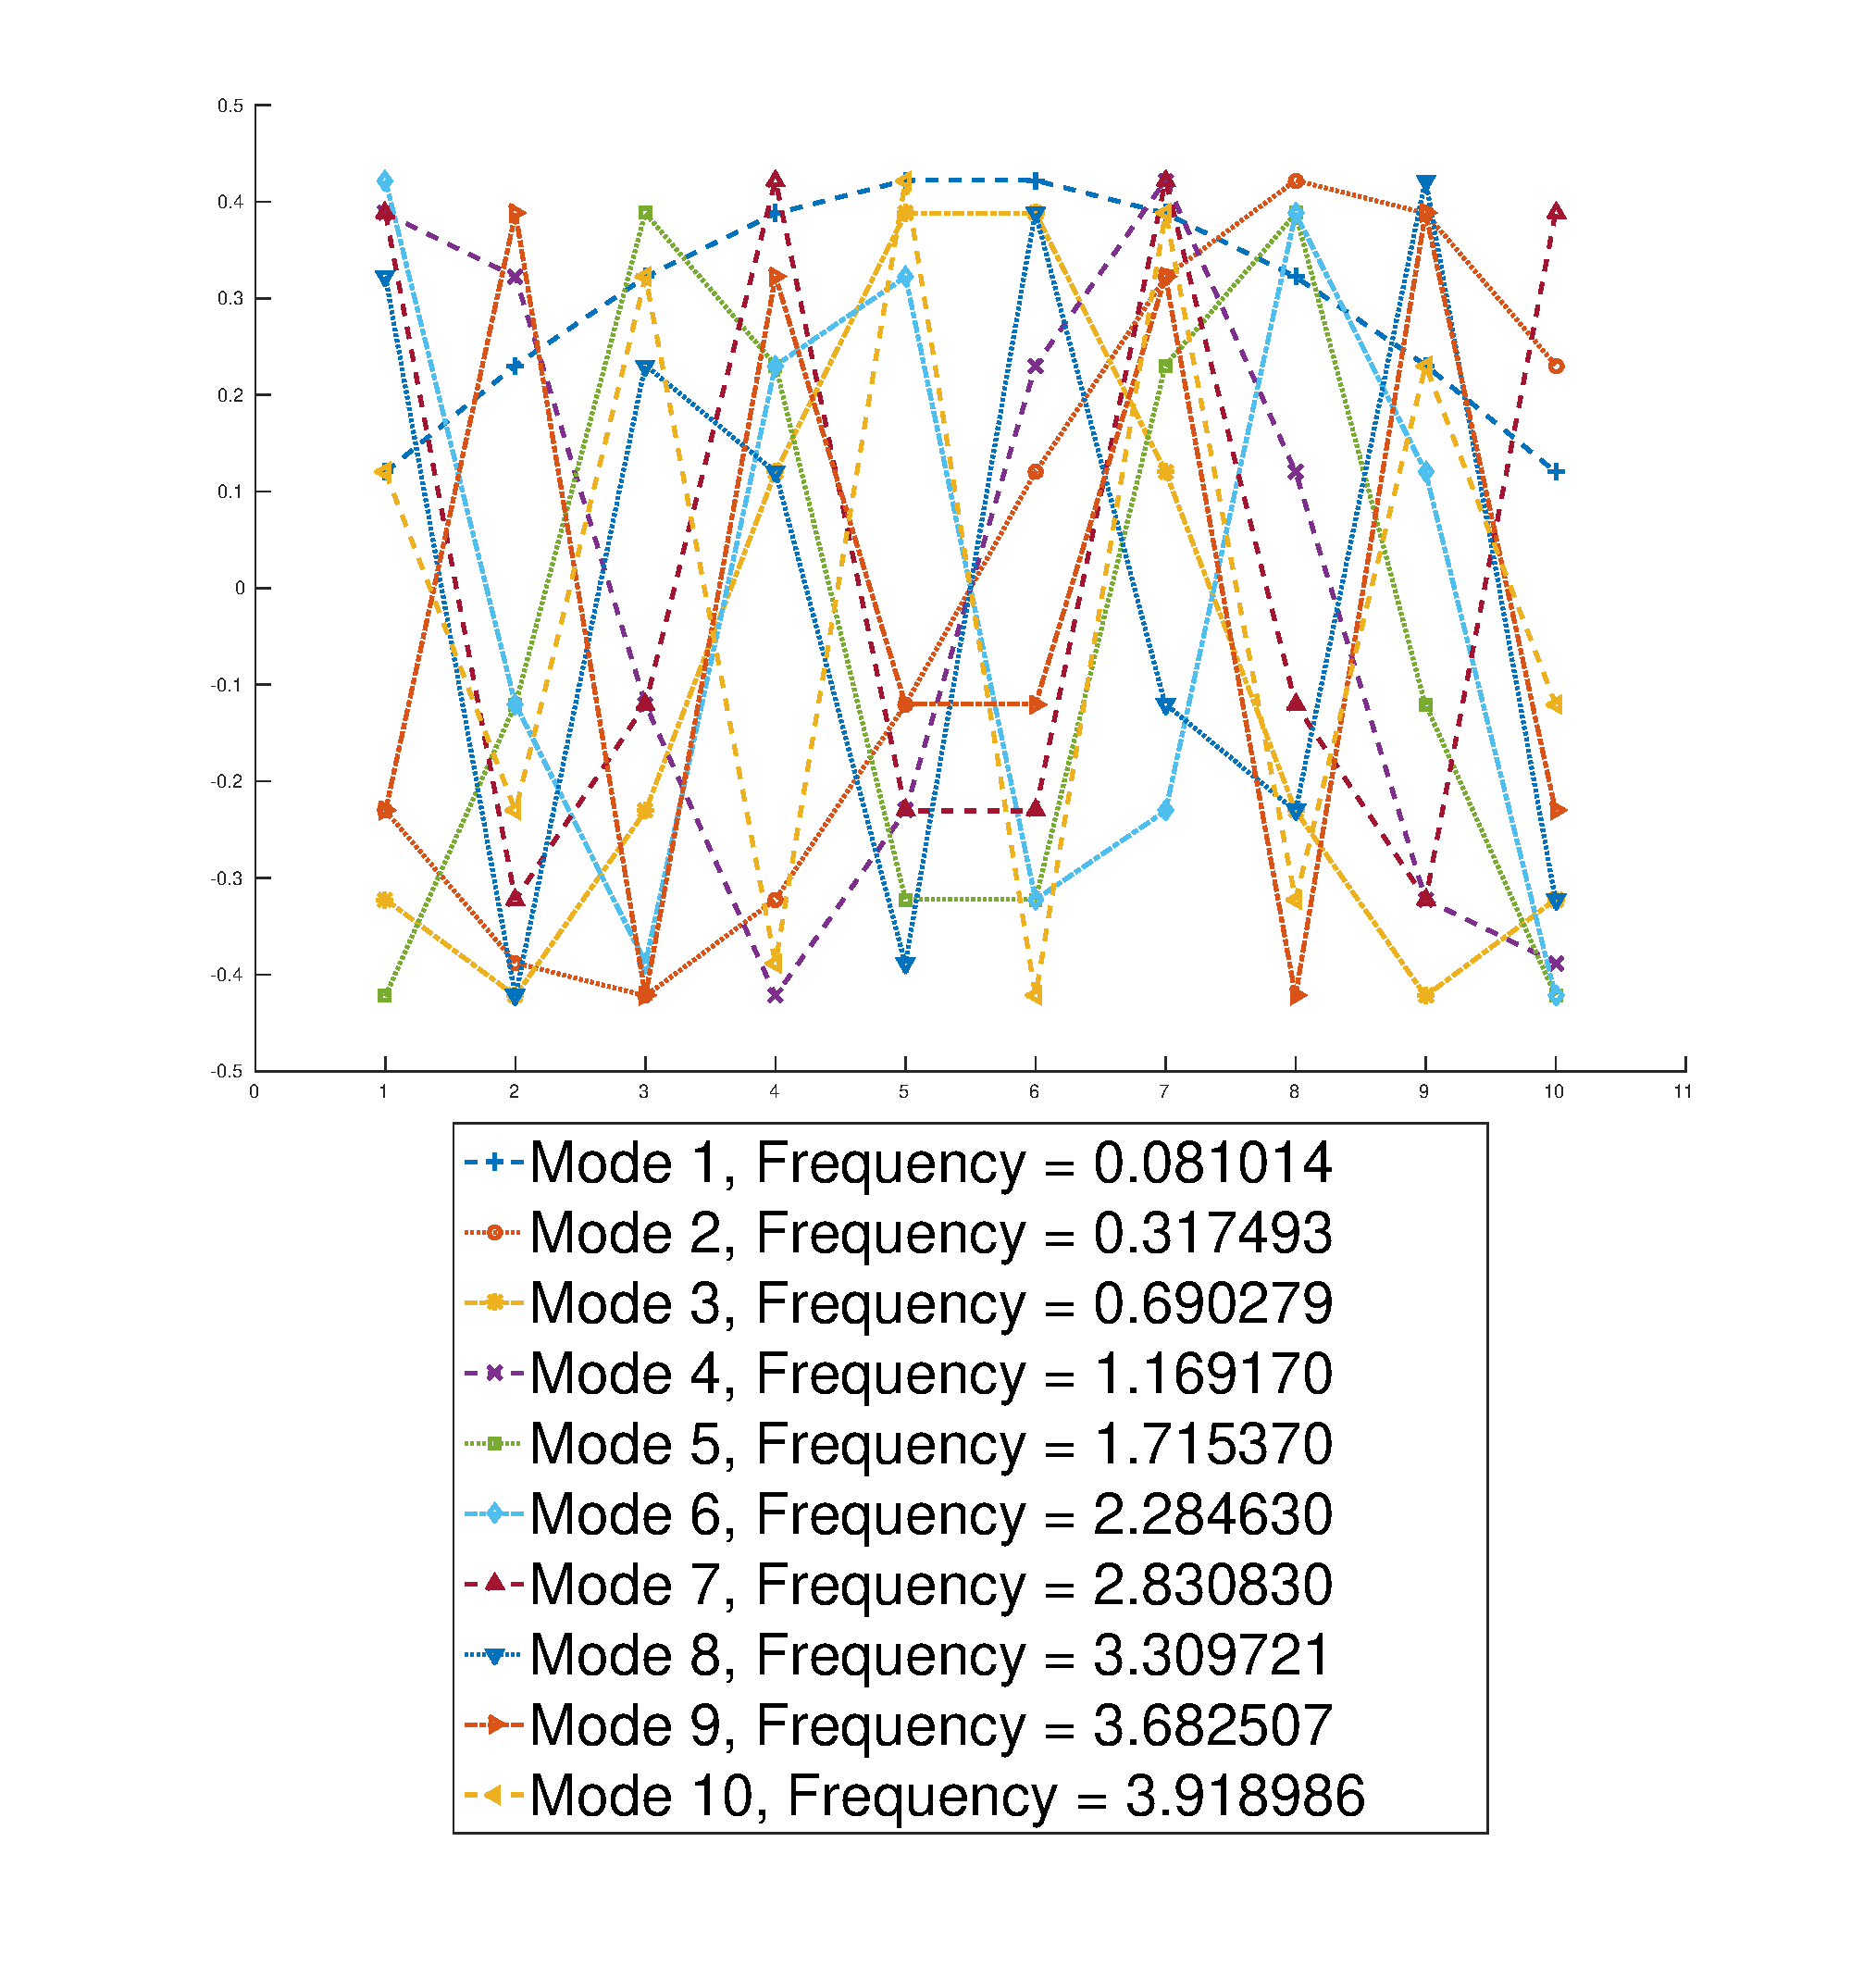
\includegraphics[width=\columnwidth]{figures/low-all.eps}
	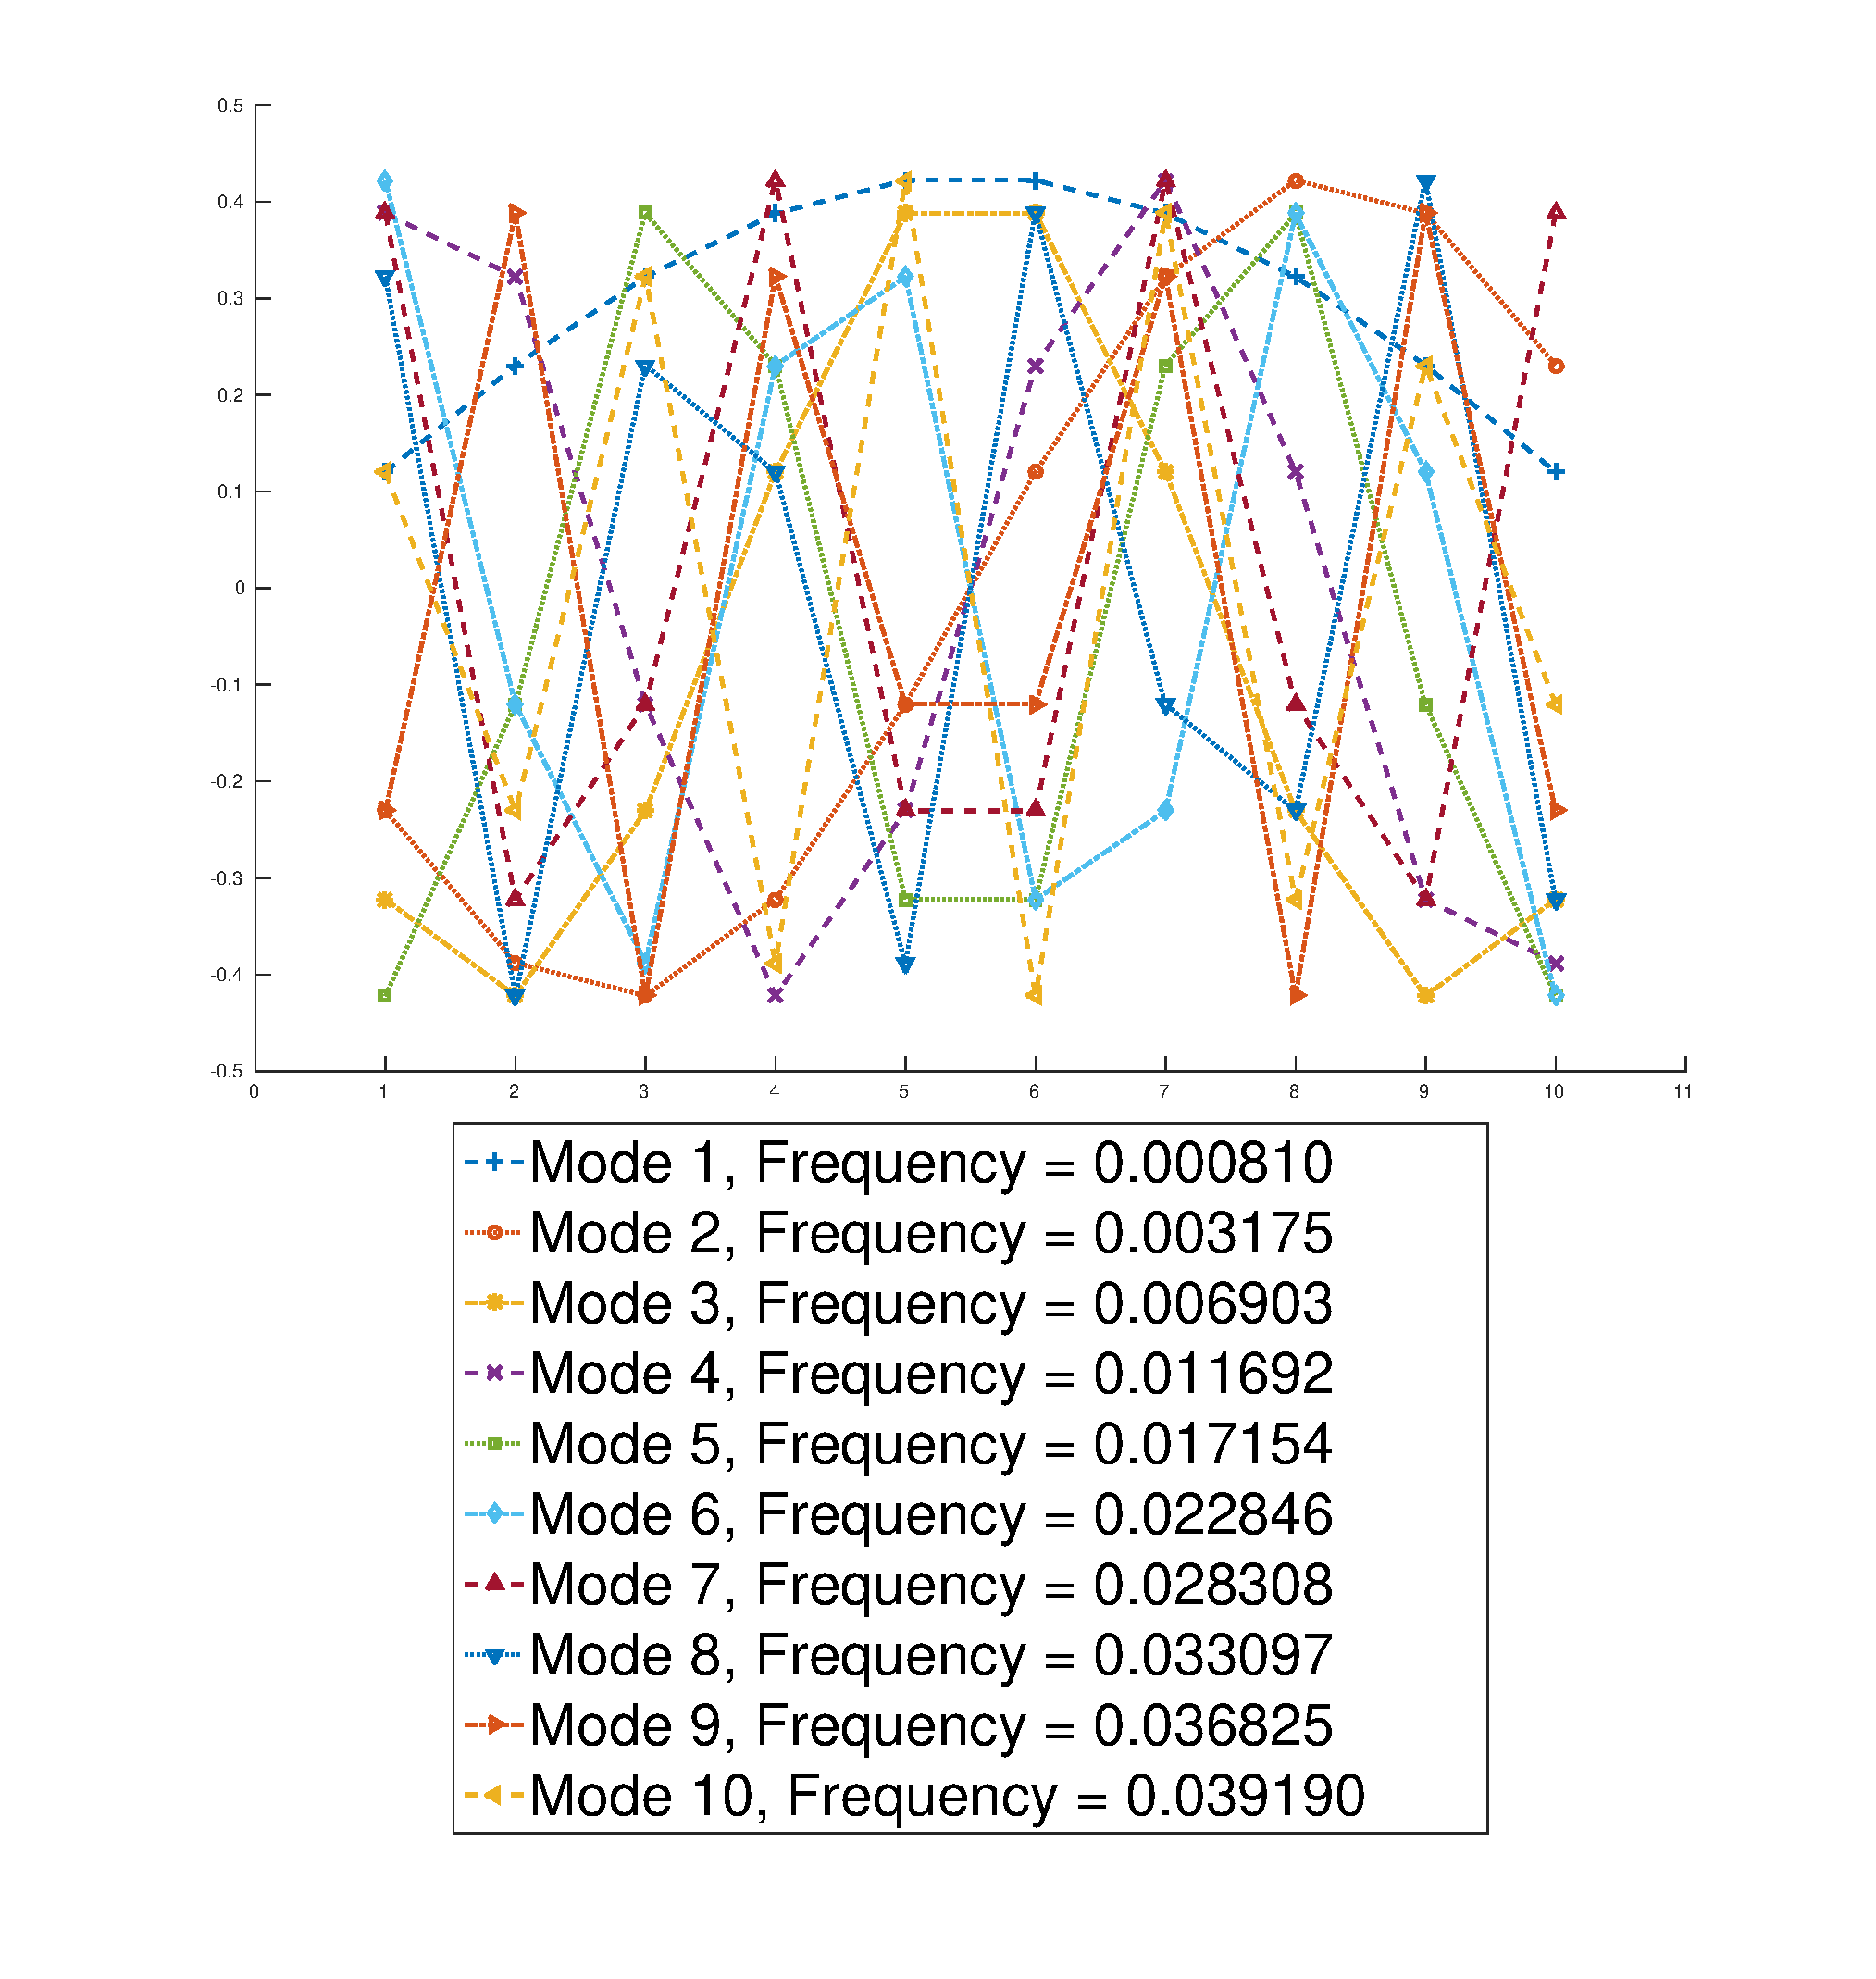
\includegraphics[width=\columnwidth]{figures/high-all.eps}
	\caption{Normal Modes of All Masses $M_{\rm{Low}}$ (Top) and $M_{\rm{High}}$ (Bottom)}
	\label{fig: constant-mass}
\end{figure}

\Cref{fig: constant-mass} shows how the string responds when masses are places evenly across the string. The natural modes are exactly the same, but the frequency is divided by the mmultiplier of the masses. This indicates that we could achieve a certain set of frequencies within a given error by scaling the masses by a certain amount. There is also a good amount of variation in the eigenmodes and it would be suspected that using more masses could provide access to a broader range of frequencies. This case could be used to systematically place masses to achieve a set of desired frequencies.

We will now look at placing different masses around the string. To achieve this, the an array of masses was created with the MATLAB command \lstinline[language=Matlab]|rand(10,1)|, creating 10 random masses -- this command could be used with another number replacing 10 to create any number of masses.

\begin{figure}[H]
	\centering
	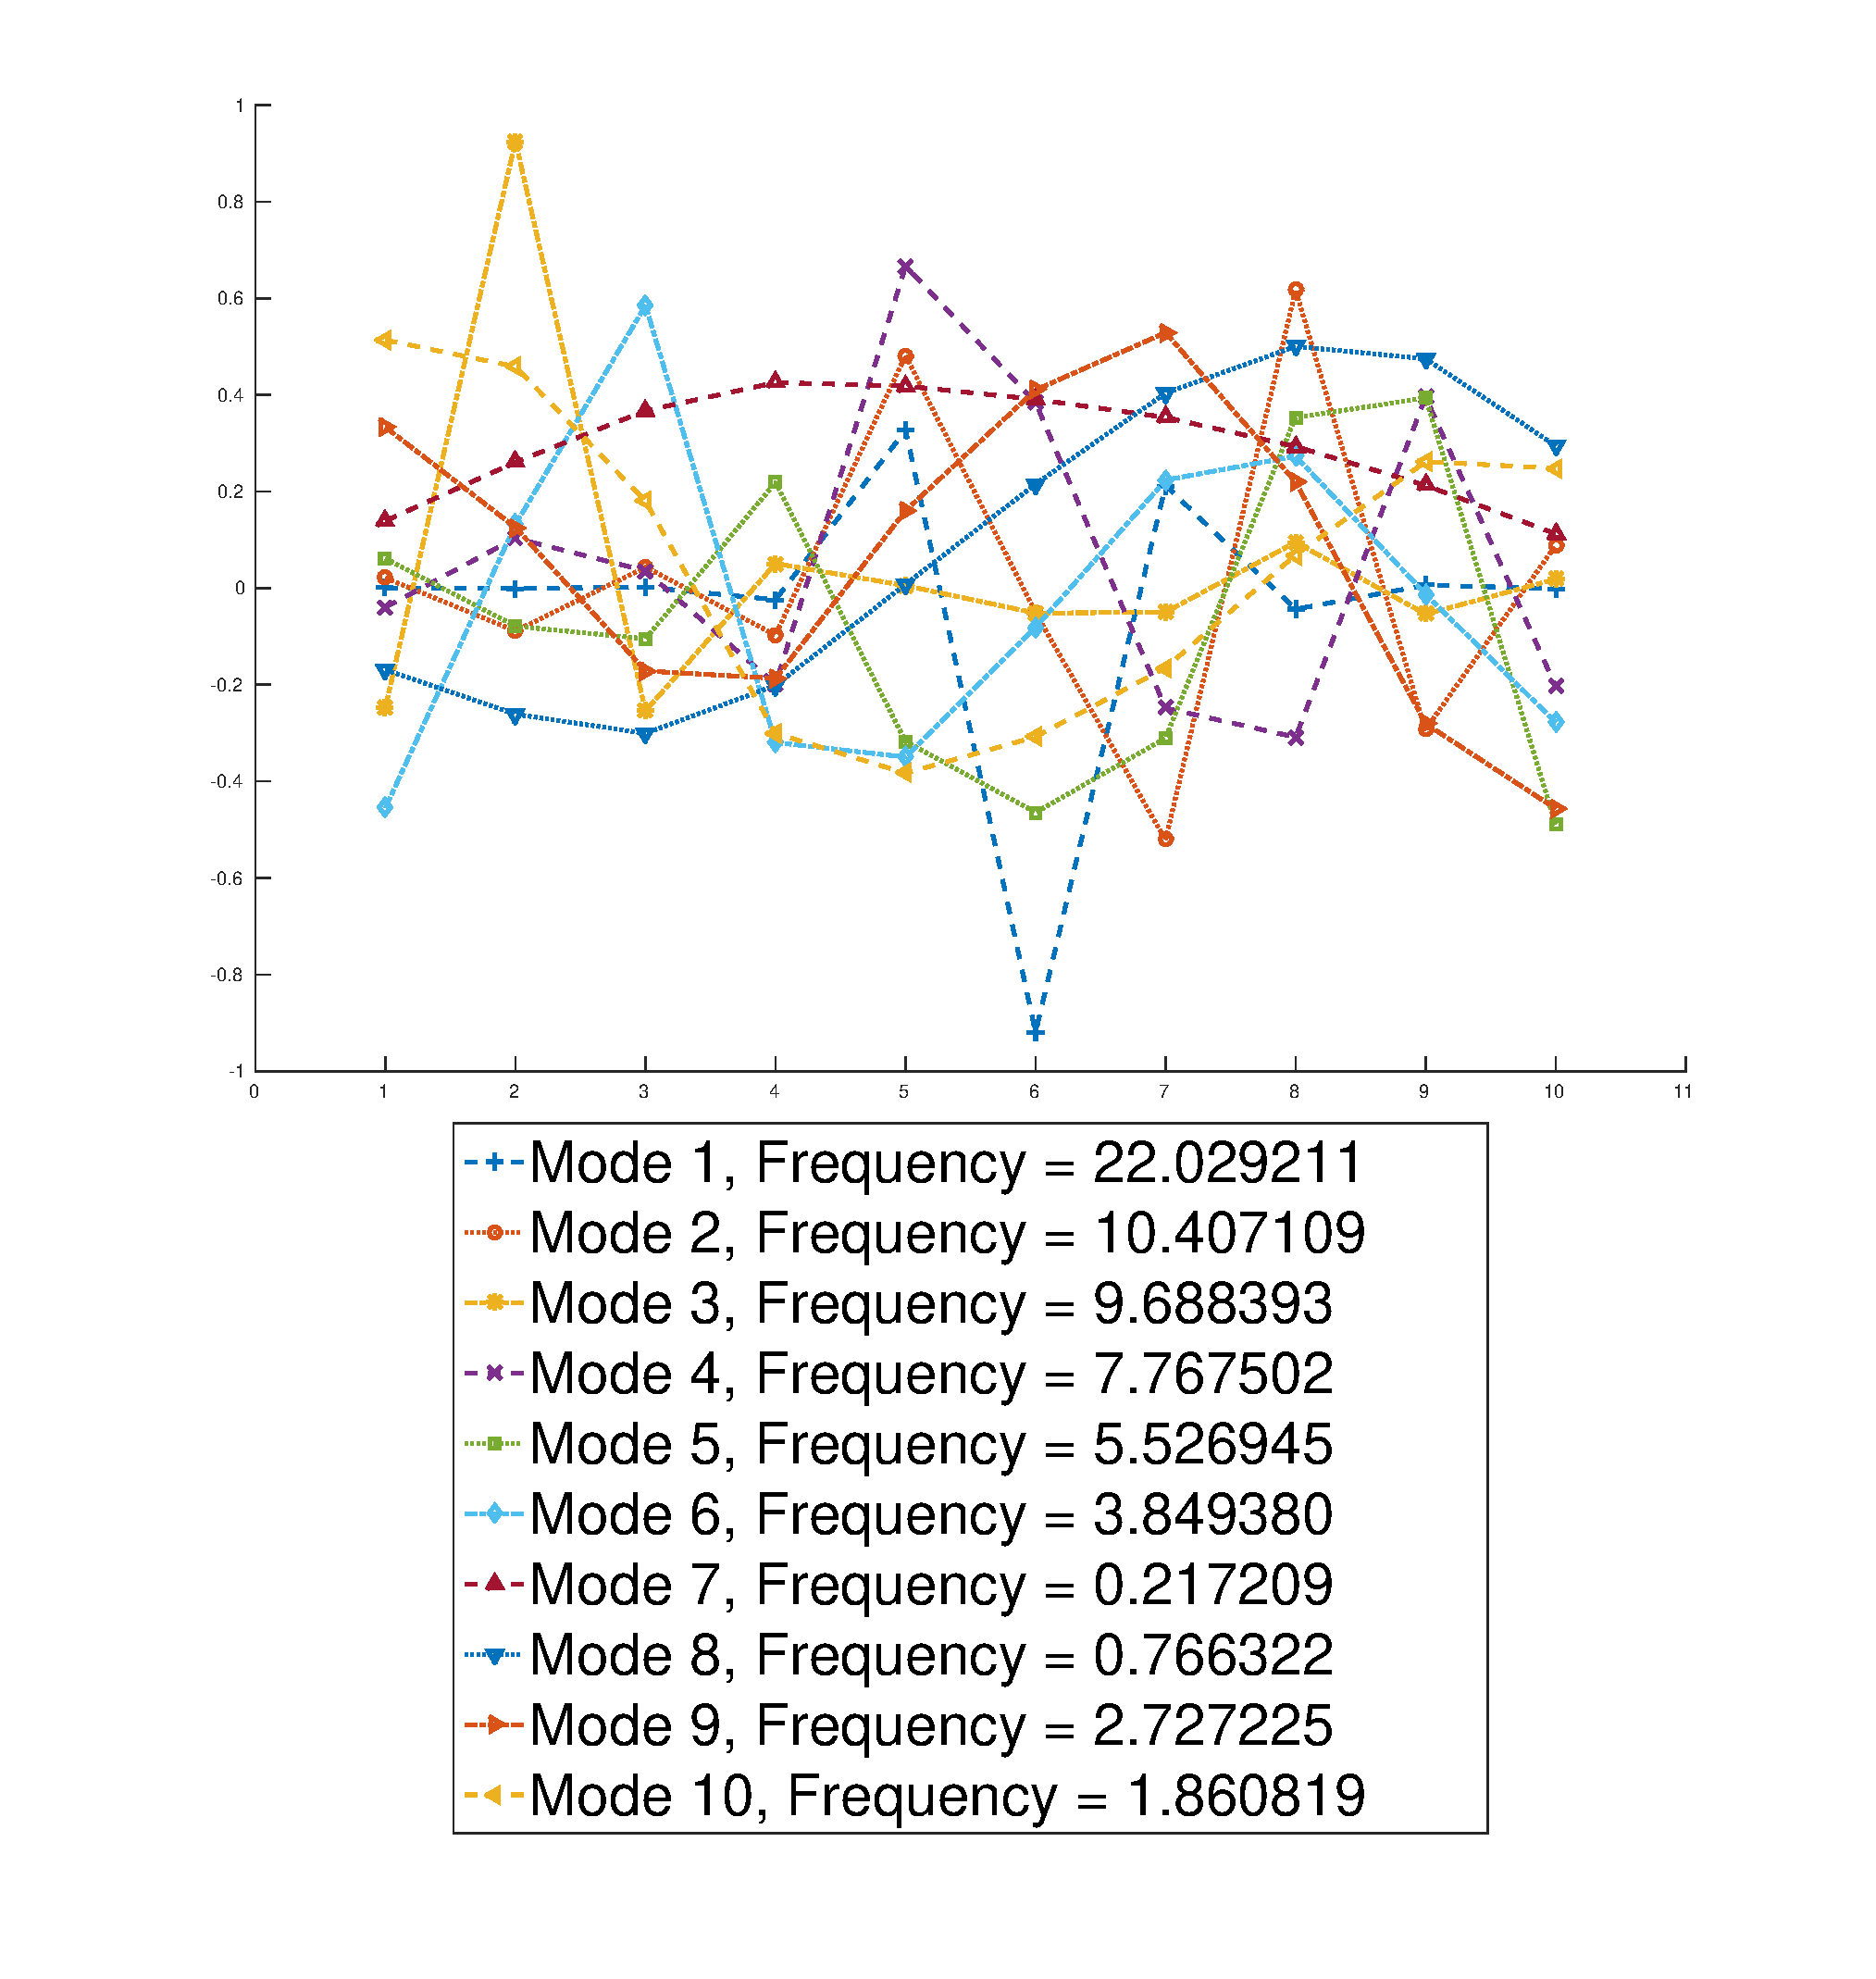
\includegraphics[width=\columnwidth]{figures/random10_1.eps}
	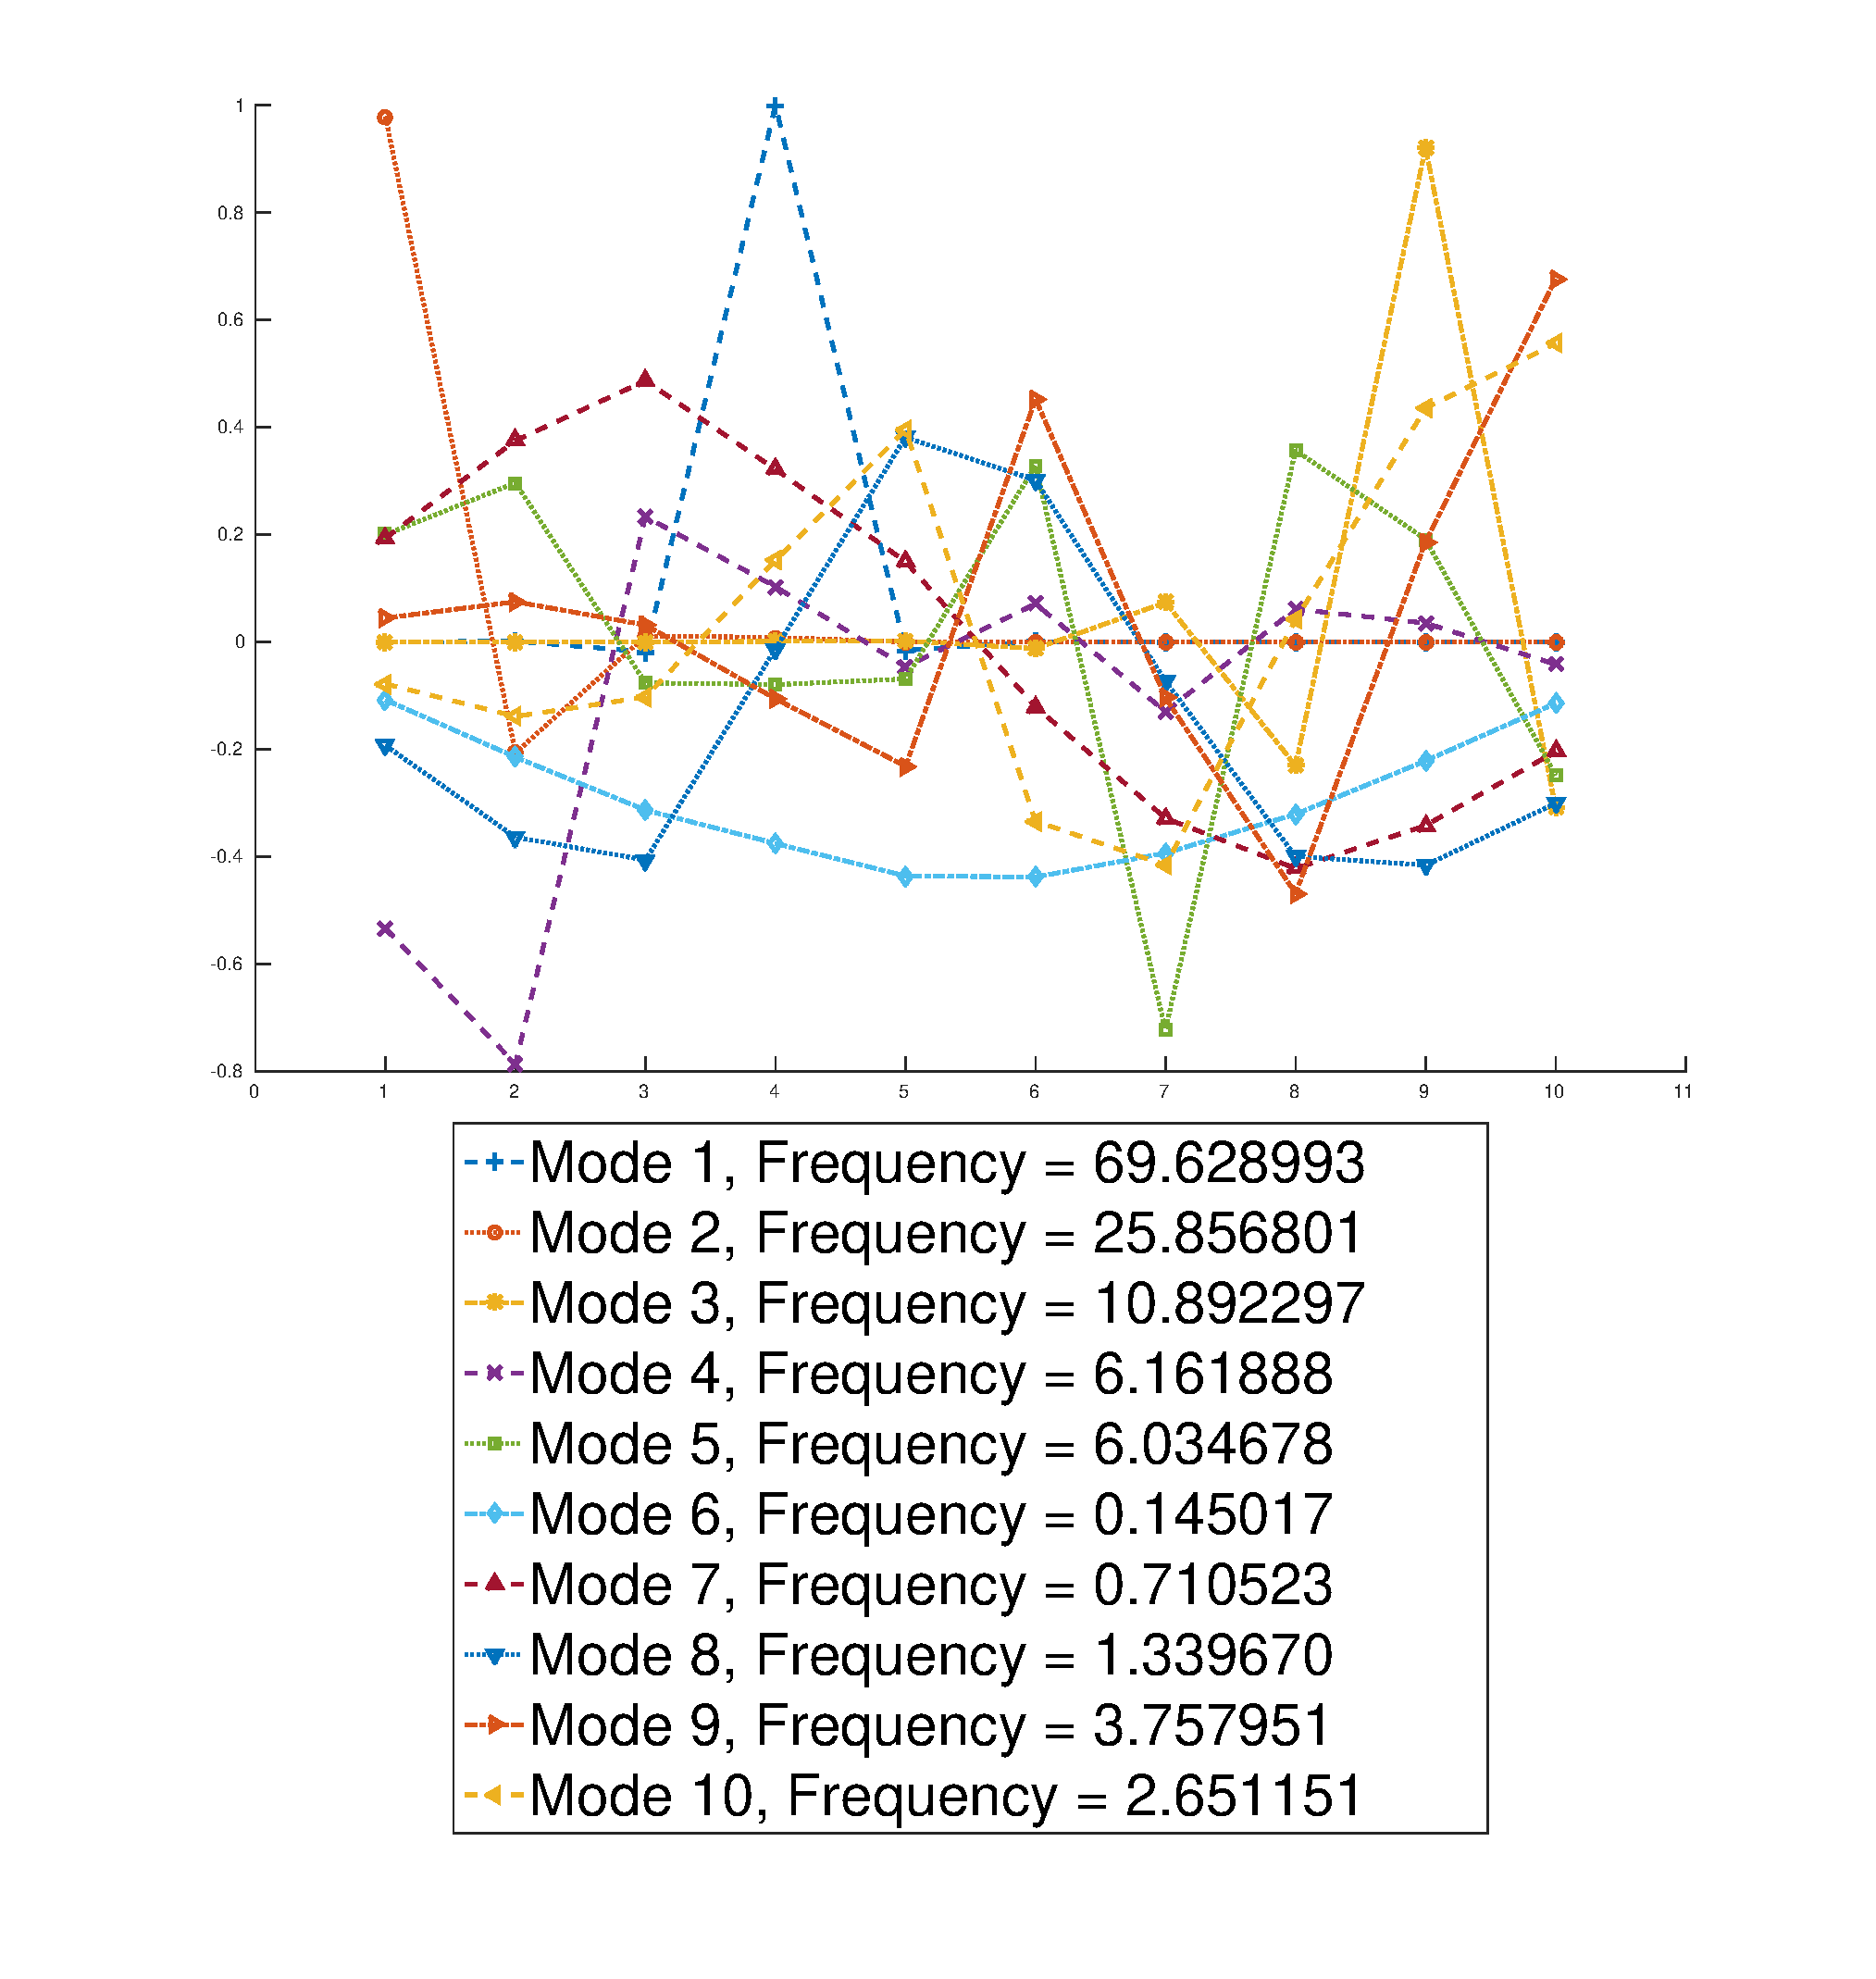
\includegraphics[width=\columnwidth]{figures/random10_2.eps}
	\caption{Normal Modes of 2 Sets of 10 Random Masses}
	\label{fig: random10}
\end{figure}

As can be seen in \cref{fig: random10}, the normal (natural) modes of masses placed randomly on a string is very chaotic. Due to the randomness of the normal modes and variations of frequencies of the modes, it is likely that a very broad range of motion may be formed by these normal modes; however, it would be very unwise to randomly generate masses until a desired set of frequencies is reached.

We can also explore the effect of placing the same masses in a variety of configurations. In this exploration, we will consider two sets of equal masses, $M_{\rm{Low}} = 1$ and $M_{\rm{High}} = 100$ respectively representing small and large masses. We will explore the low and high masses being placed on opposite sides of the string, as well as the low and high masses being places on one side of the string with random masses on the other side, using $M_{\rm{Low}}$ and $M_{\rm{High}}$ as multipliers for the random masses where $M_{\rm{Random}} \in \left[0,1\right]$ before being multiplied by $M_{\rm{Low}}$ or $M_{\rm{High}}$. Once again, 10 masses will be used.

\begin{figure}[H]
	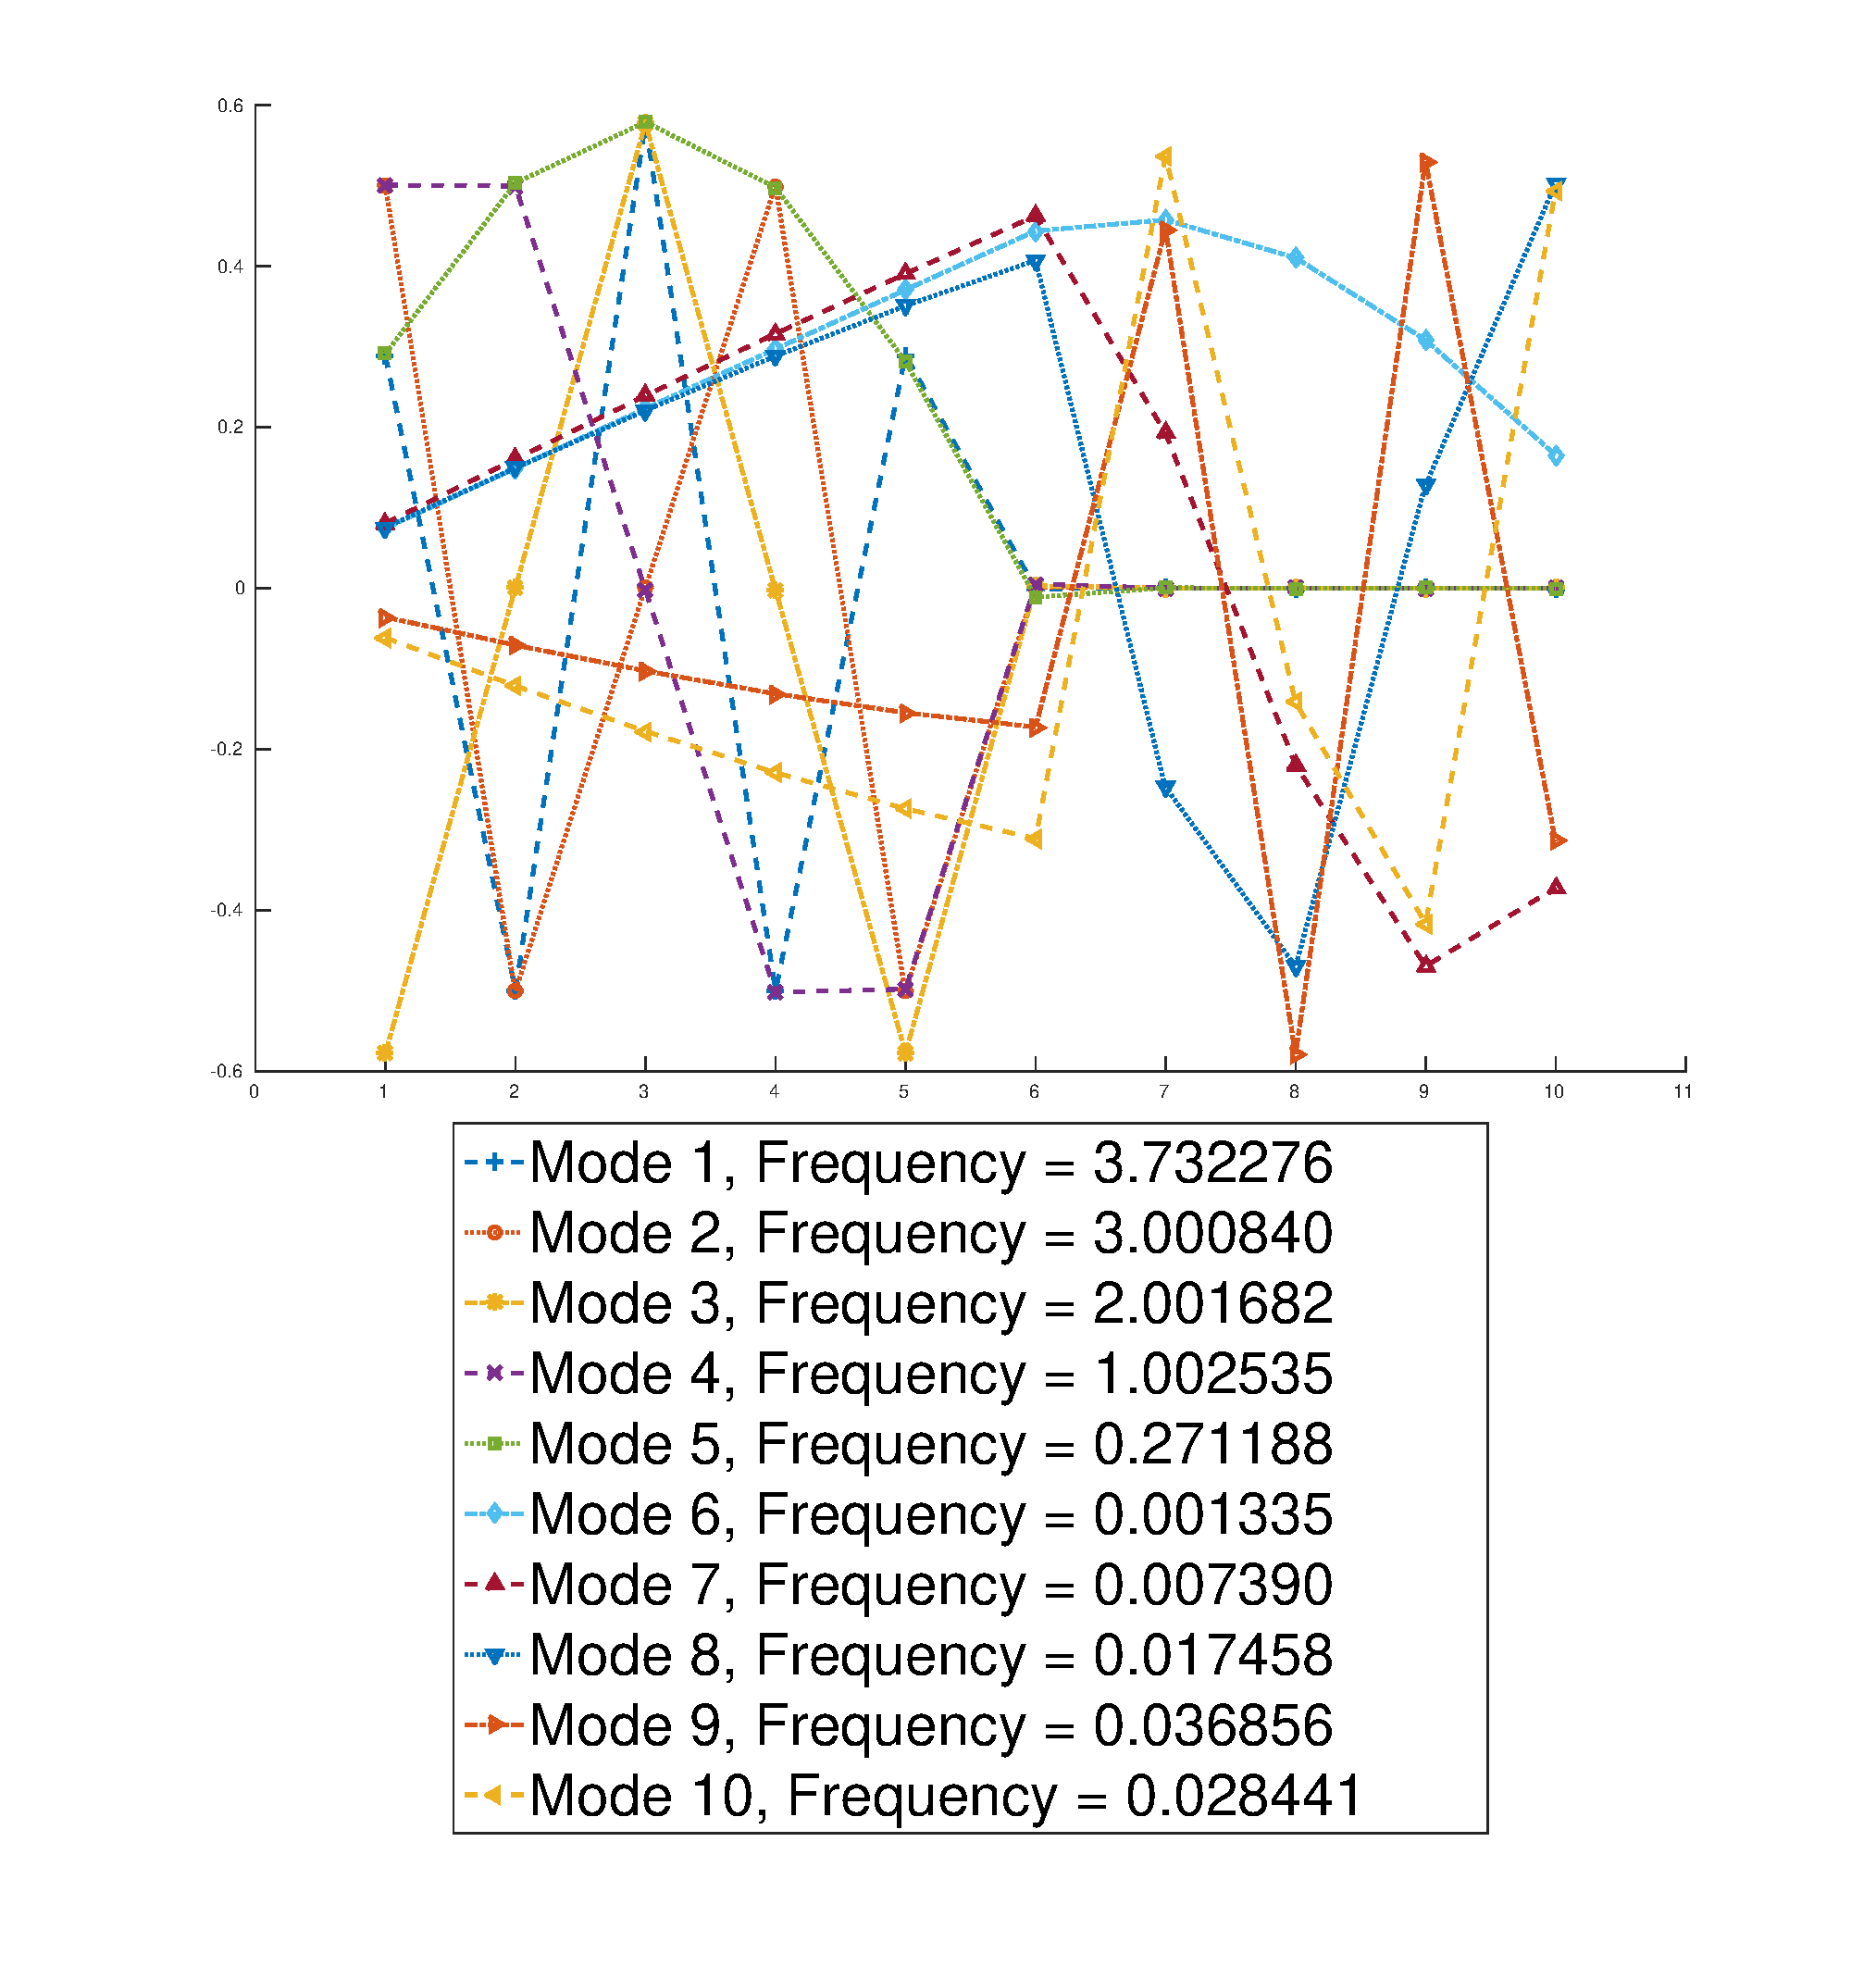
\includegraphics[width=\columnwidth]{figures/low-high}
	\caption{Normal Modes of $M_{\rm{Low}}$ on Left and $M_{\rm{High}}$ on Right}
	\label{fig: low-high}
\end{figure}

In \cref{fig: low-high}, it is seen that in all normal modes except one, primarily the smaller masses are moving, which is to be expected. There are also eigenmodes in which the smaller masses all move in a certain way, producing more movement of the larger masses; however, these are the less frequent eigenmodes.

We will now look at the effects of using constant masses with either high or low random masses on the other sides. 

\begin{figure}[H]
	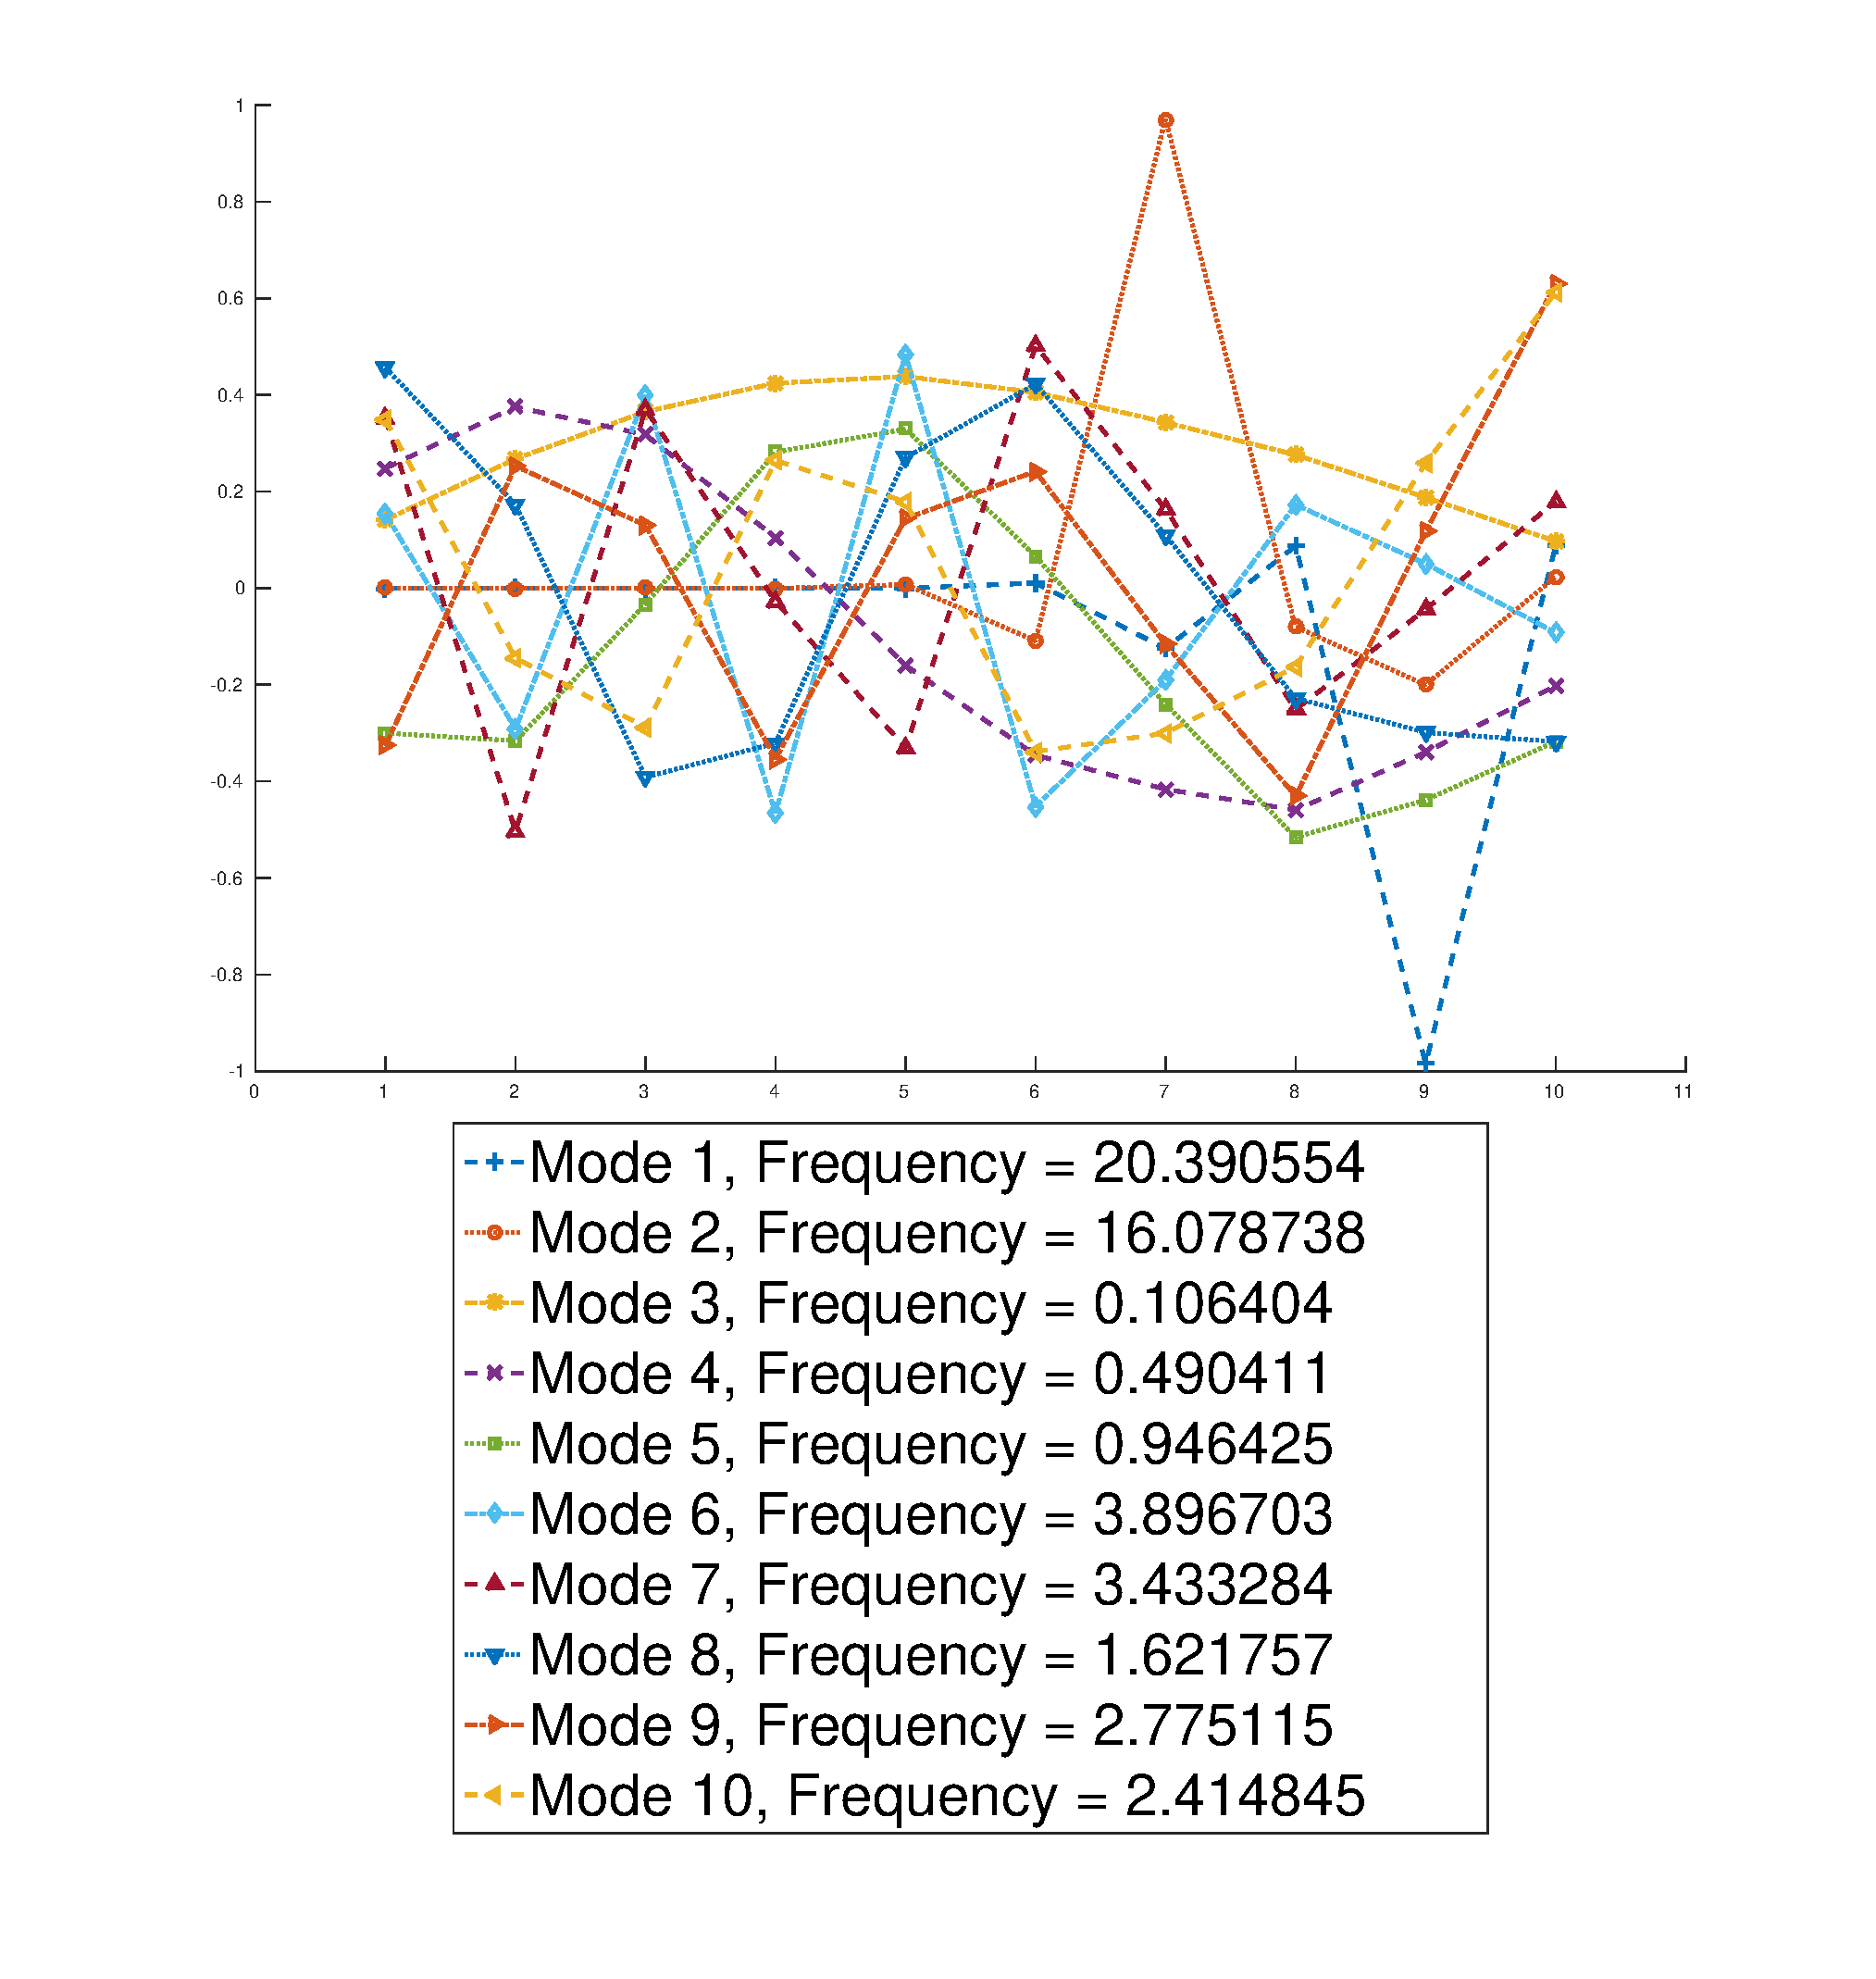
\includegraphics[width=\columnwidth]{figures/low-lowrand.eps}
	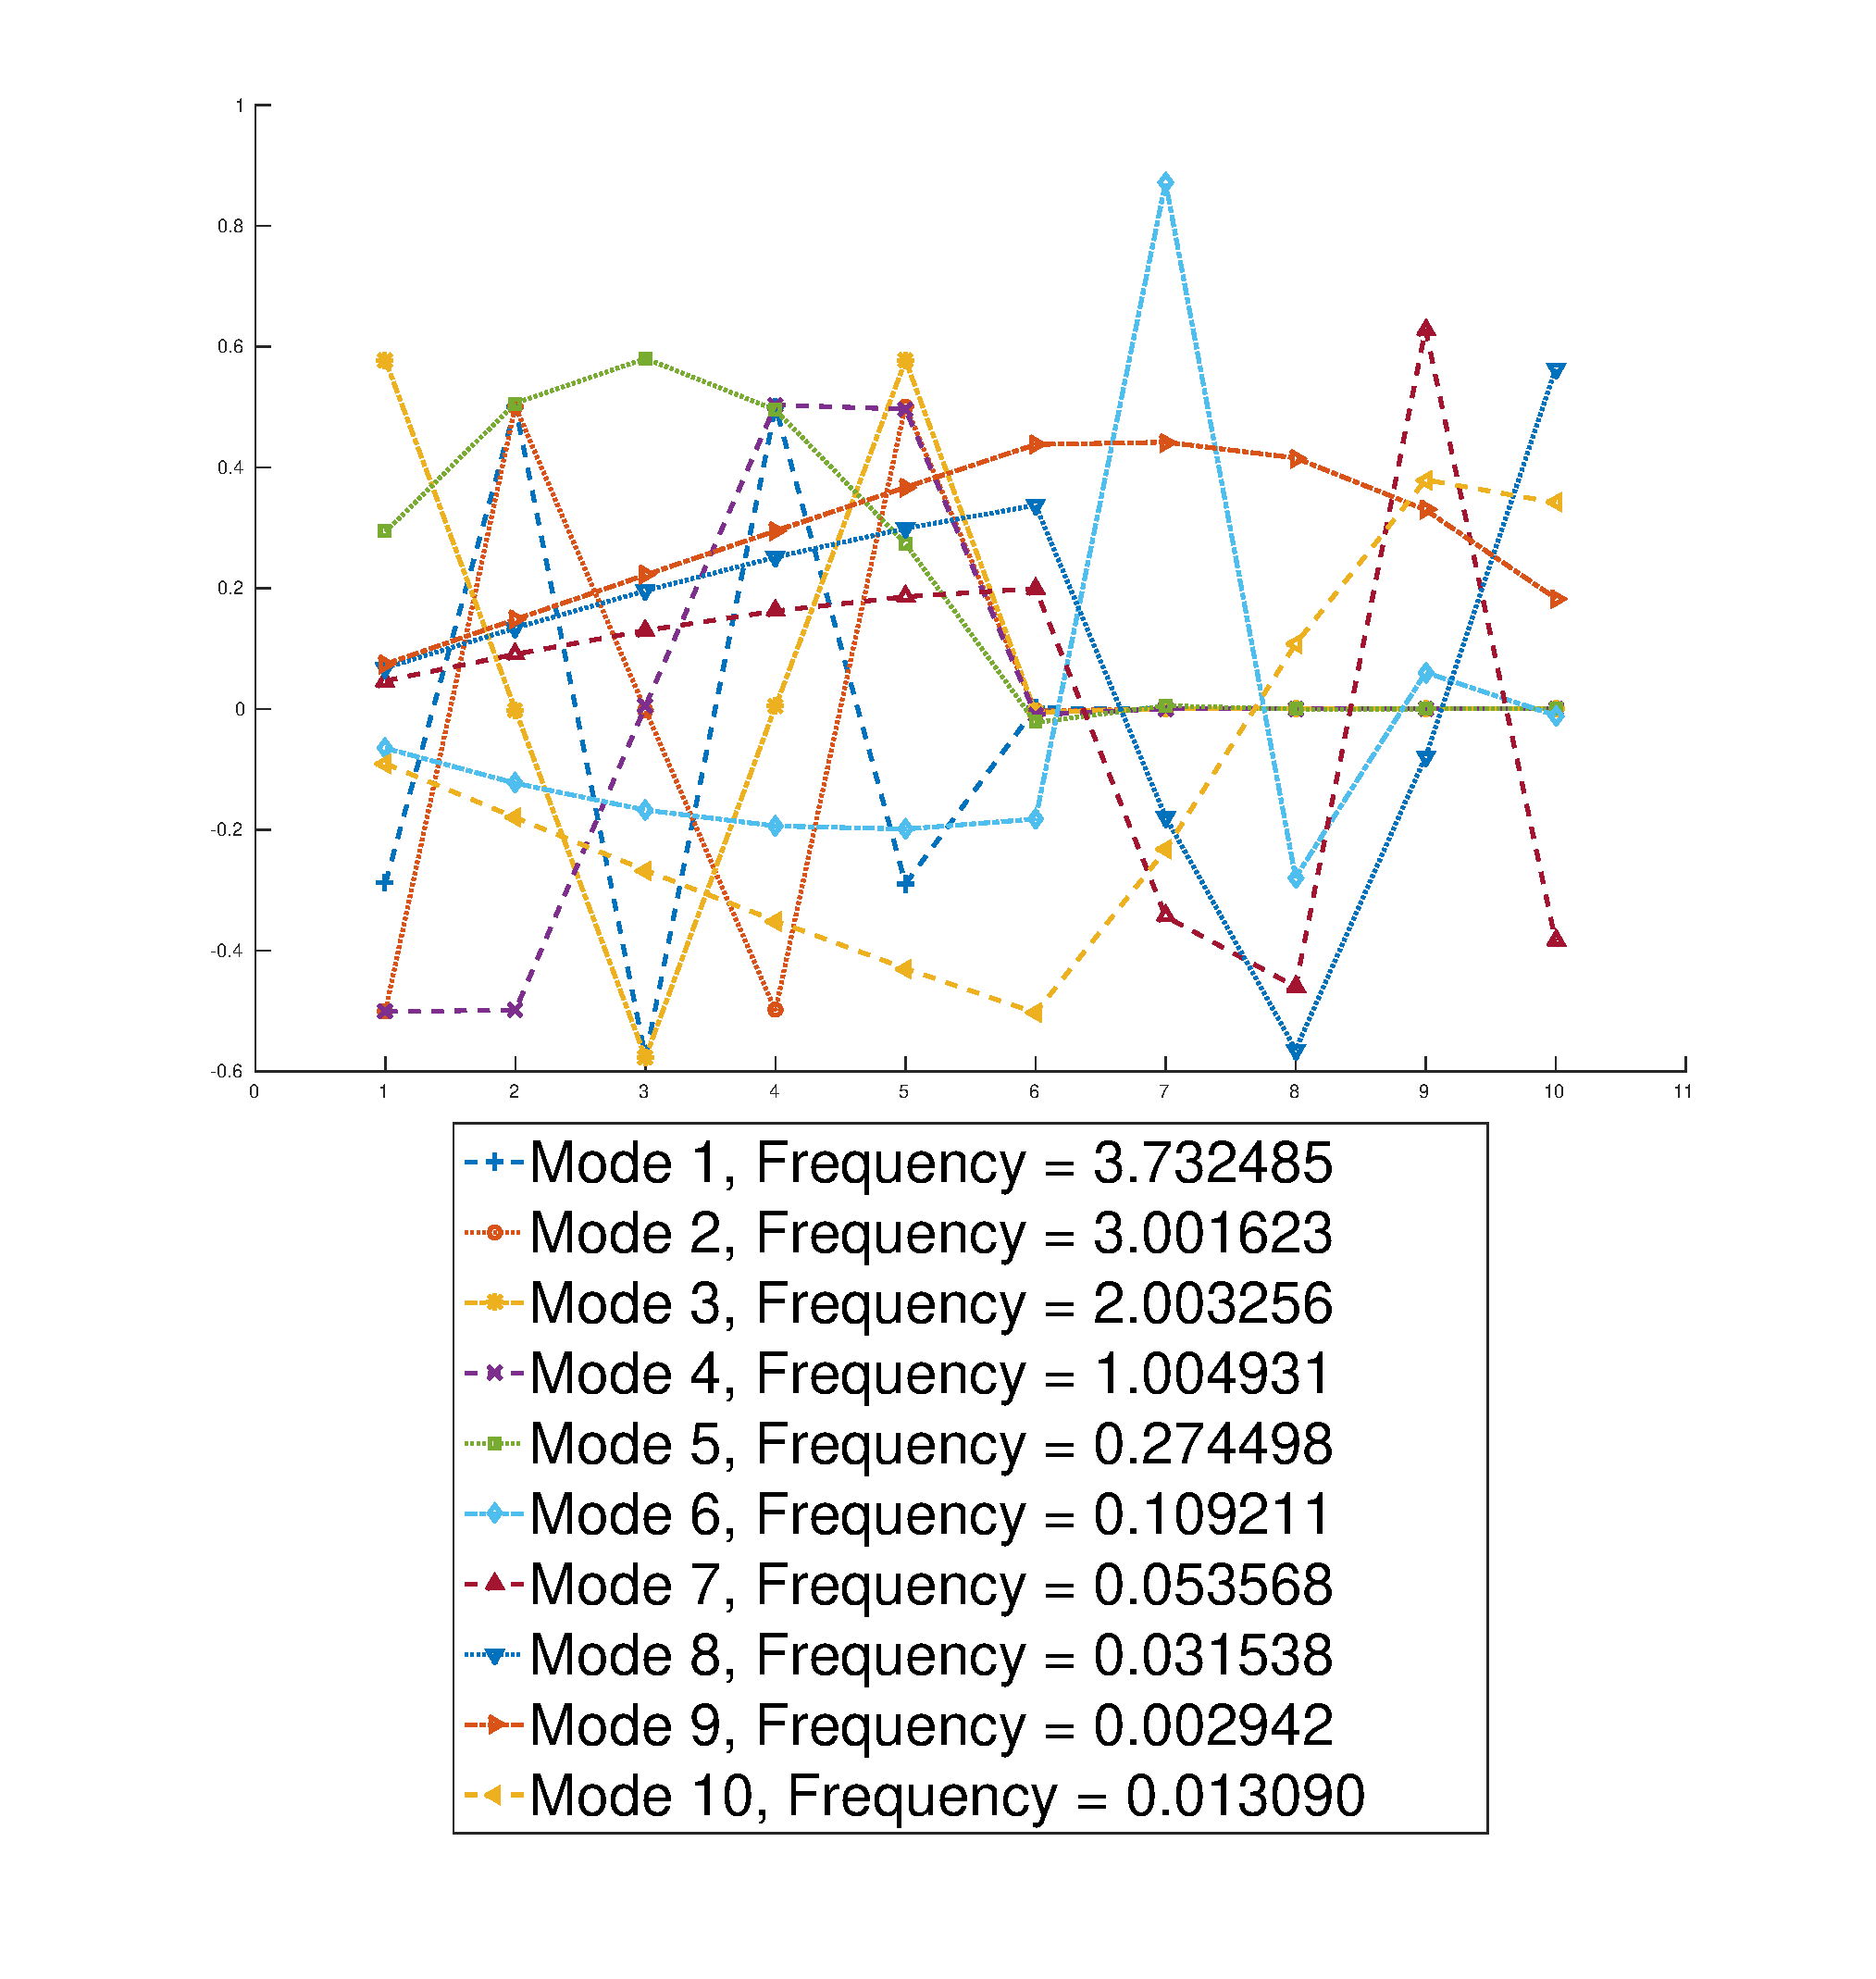
\includegraphics[width=\columnwidth]{figures/low-highrand.eps}
	\caption{Low Masses on Left with Low (Top) and High (Bottom) Random Masses on Right}
	\label{fig: low-rand}
\end{figure}

\Cref{fig: low-rand} shows the effects of random masses on the oppopsite side of a string from low masses. These plots can be compared with the plots in \cref{fig: high-rand}. It can be seen that the modes in all cases are quite chaotic. Having a chaotic system such as this would allow for constructing arbitrary frequencies, although it would once again be unwise to generate random masses until the desired set of frequencies is achieved.

\begin{figure}[H]
	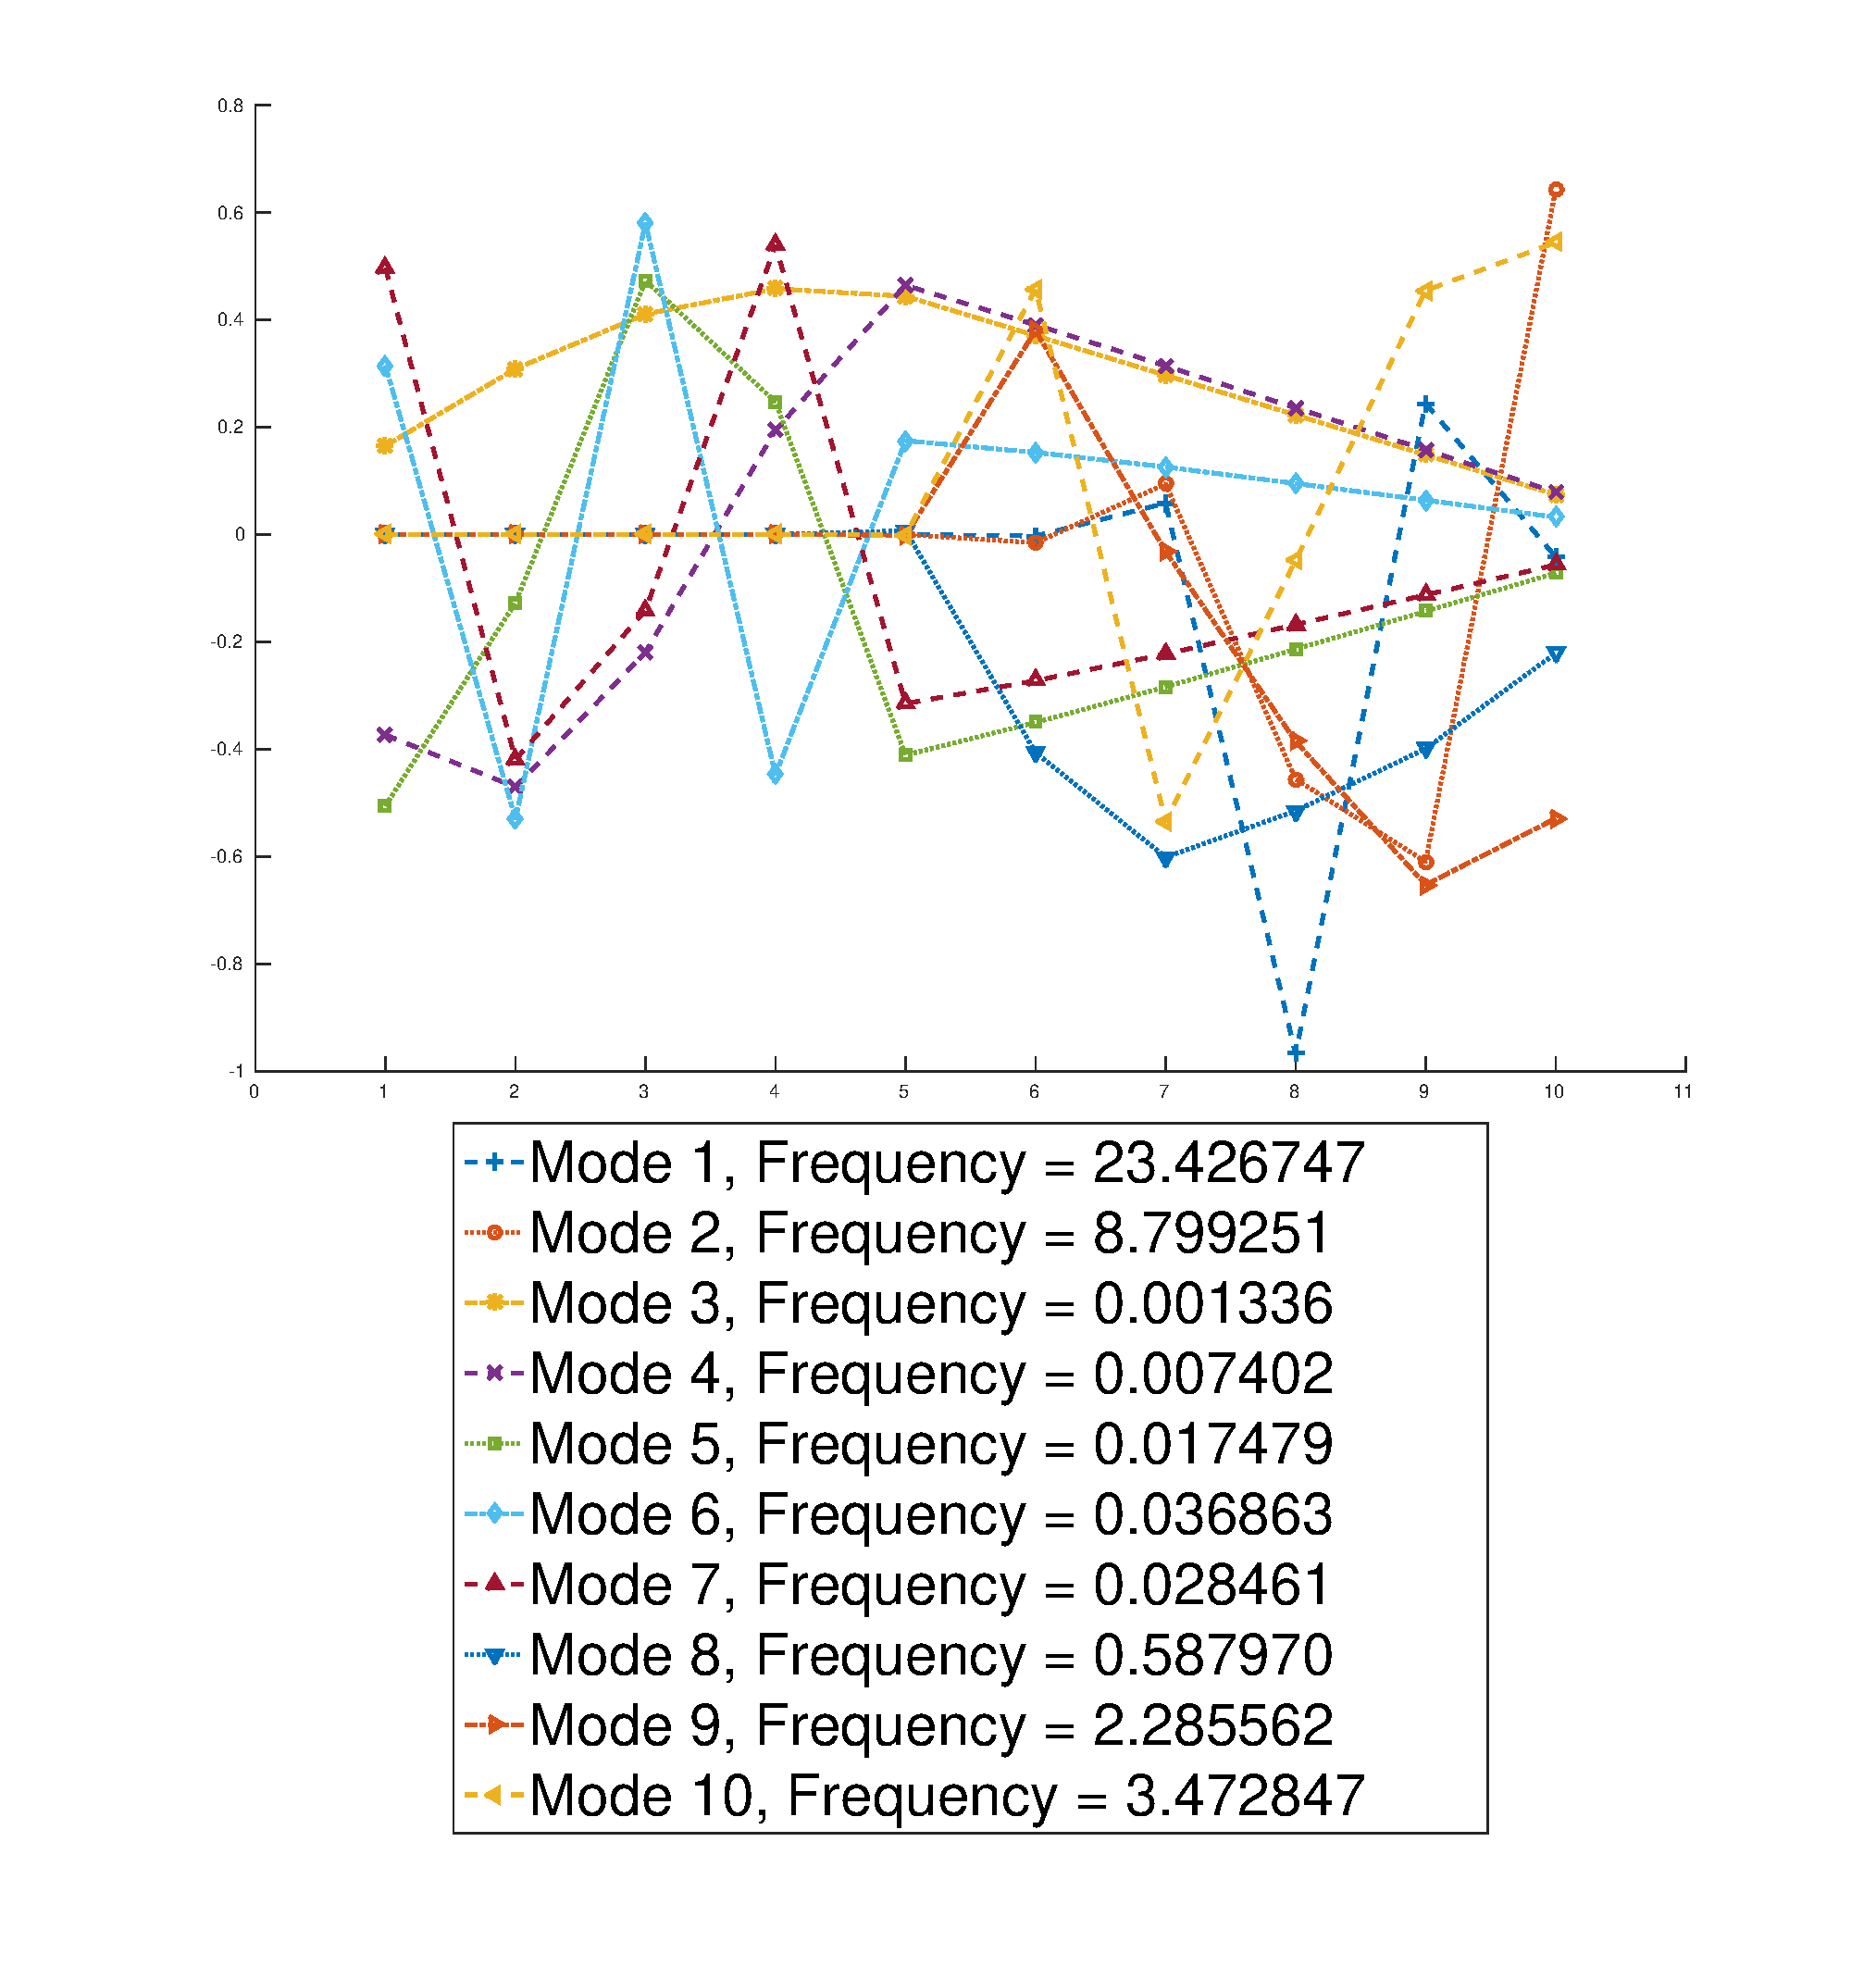
\includegraphics[width=\columnwidth]{figures/high-lowrand.eps}
	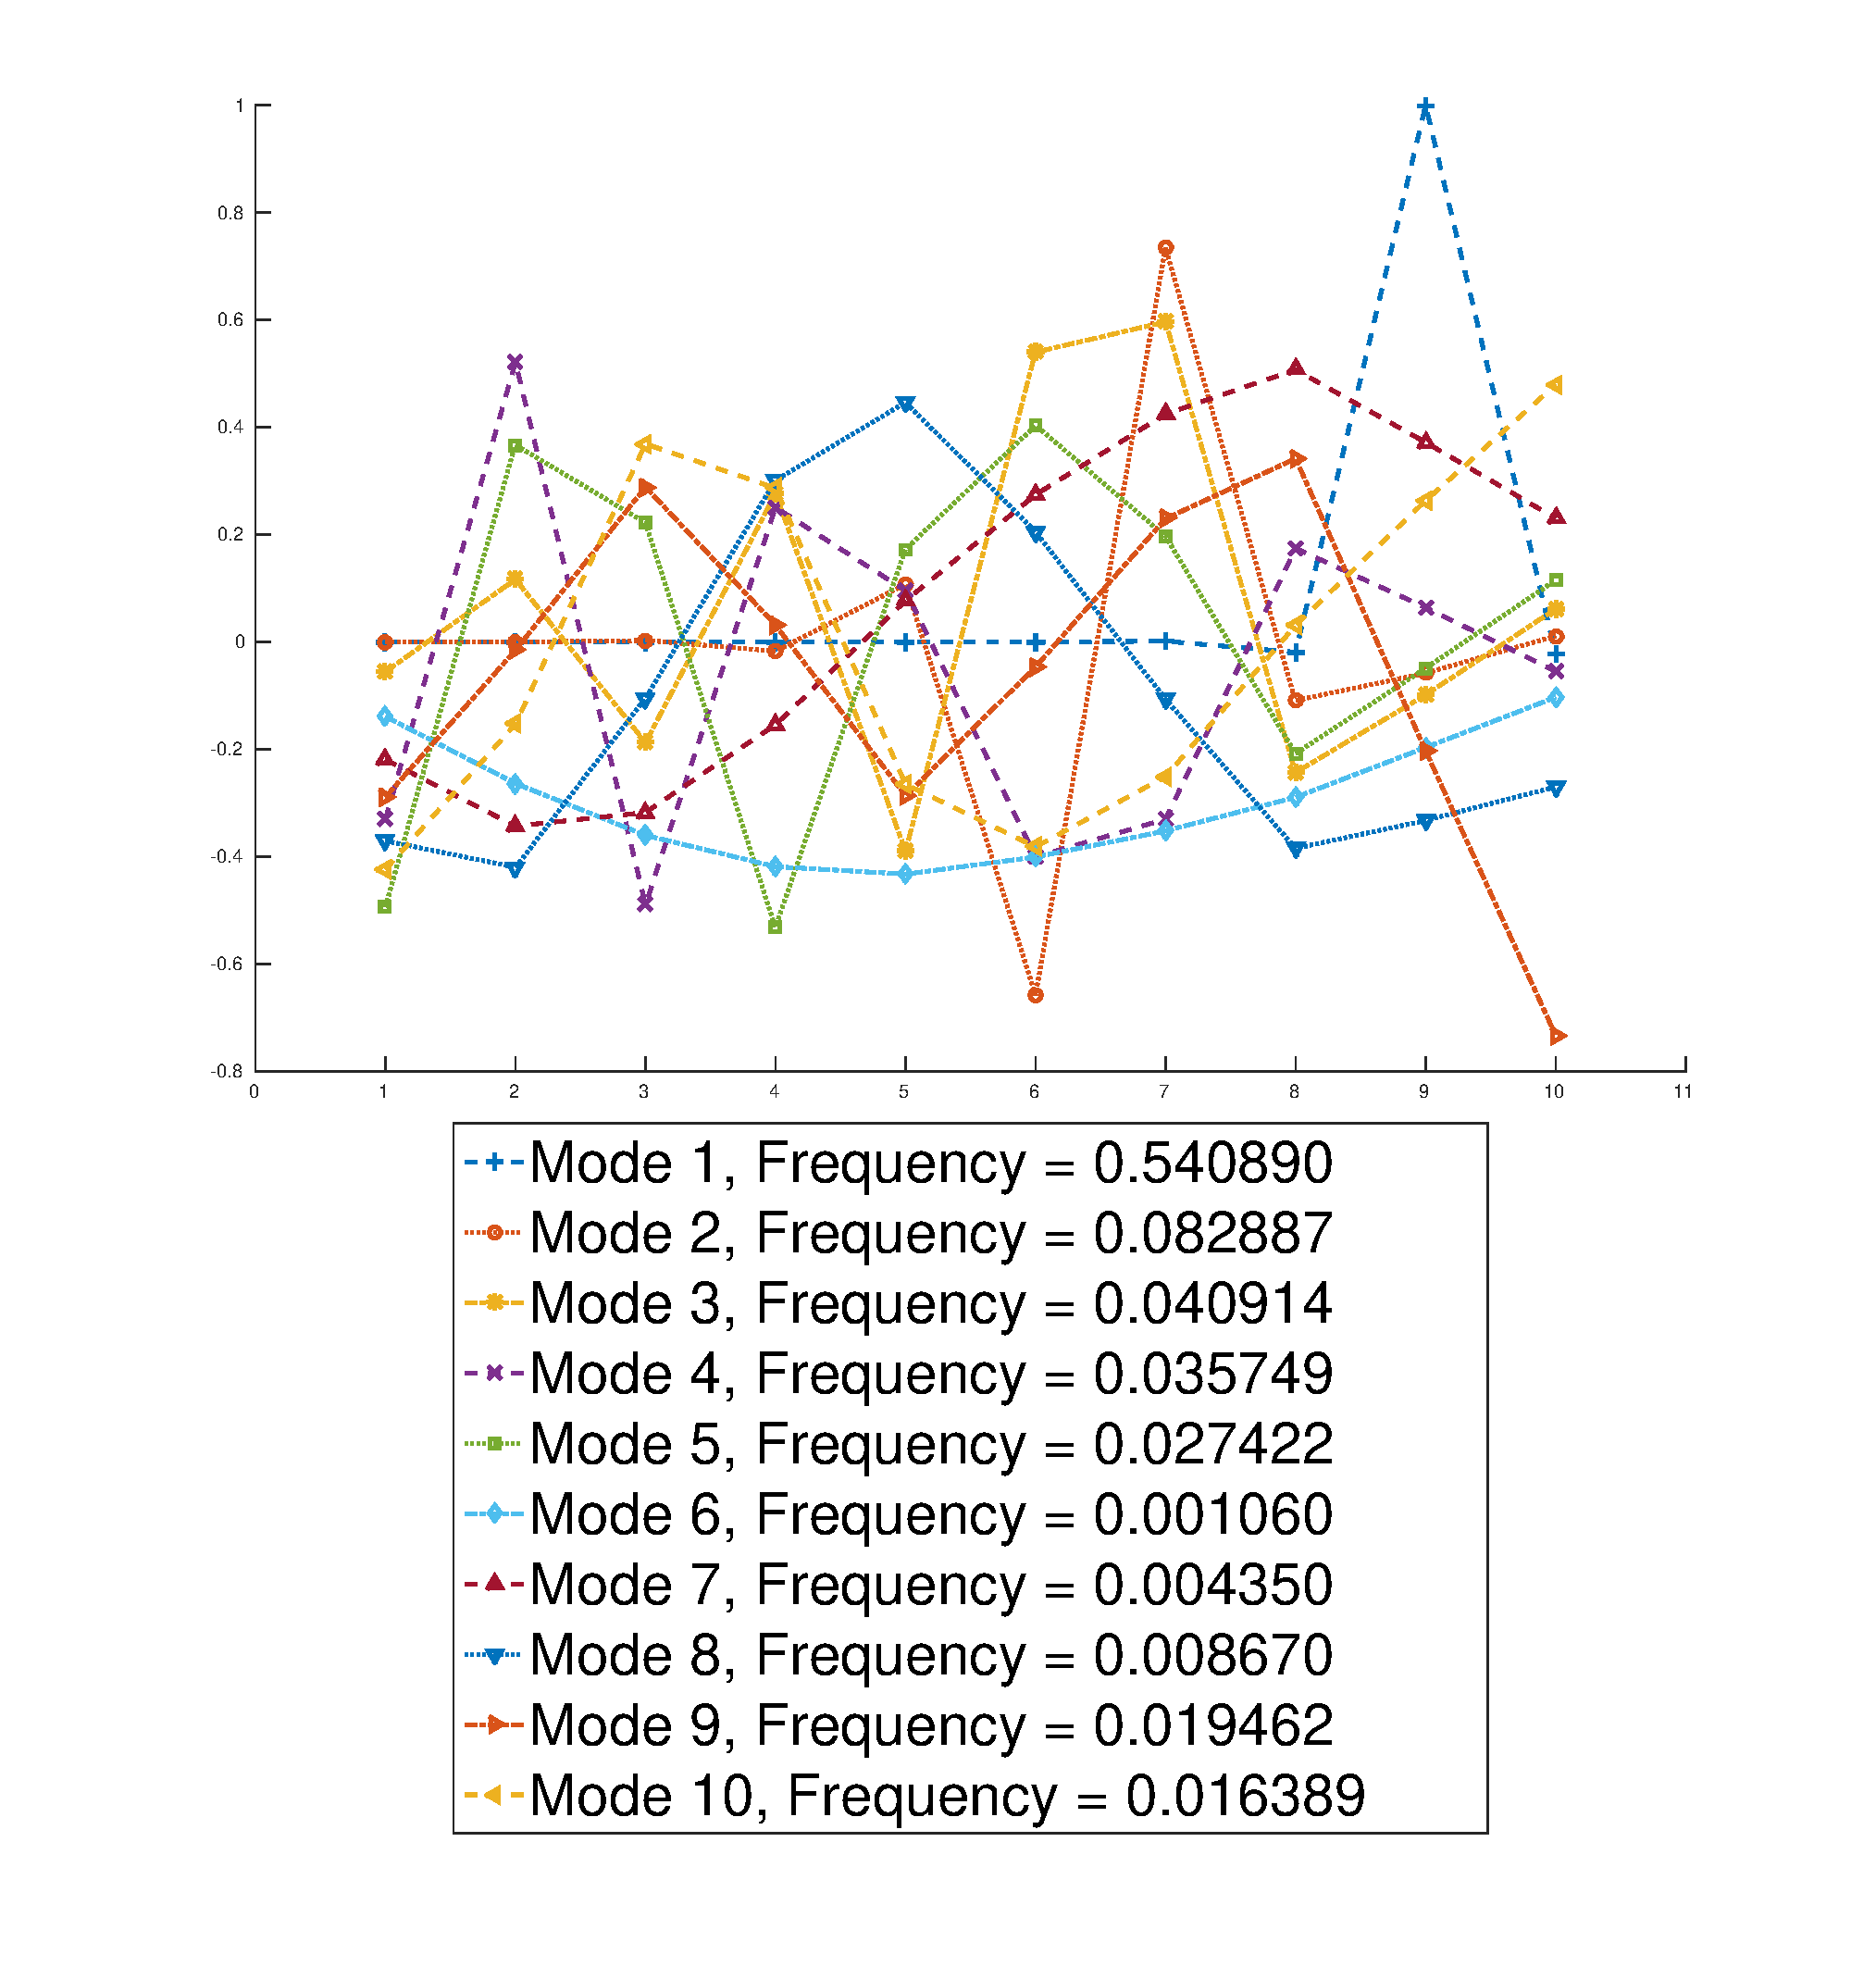
\includegraphics[width=\columnwidth]{figures/high-highrand.eps}
	\caption{High Masses on Left with Low (Top) and High (Bottom) Random Masses on Right}
	\label{fig: high-rand}	
\end{figure}

From this exploration of the inverse eigenvalue problem, it seems that frequencies in general are quite arbitrary when the parameters of a system are able to be changed. However, for a given physical system, such as a violin, the modes and frequencies are already determined. Furthermore, in a system such as a violin, the masses on the string would be represented by infinitesimal mass $dm$ with width between the masses $h \to 0$. The system represented here is similar to a set of discrete masses connected by springs with the displacements of the masses $X_i$ representing the distance of the mass from the equilibrium position of the spring. It should also be noted that while there are a given number of natural modes with their respective natural frequencies, superposition of these modes also happens as a system evolves in time.

\end{multicols*}



\begin{appendices}
	\crefalias{section}{appsec}
	\section{Code Listing} \label{app: Code Listing}

	Below is a listing of the MATLAB code used in this project. The most up to date code with the code for this report and the produced figures can be accessed at \url{https://github.com/danielunderwood/string-eigenvalue-analysis} and a compiled version of the latest report can be found at \url{https://www.sharelatex.com/github/repos/danielunderwood/string-eigenvalue-analysis/builds/latest/output.pdf}.

	\lstinputlisting[language=Matlab, caption =string\_eigenvalue\_solver.m]{string_eigenvalue_solver.m}
\end{appendices}

\end{document}
